\chapter[PB-2b CHWP]{A cryogenic HWP for PB-2b}
\label{ch:chwp_design}

In order to improve instrument sensitivity, POLARBEAR-2b, the second installment of Simons Array, implements a cryogenic half-wave plate (CHWP). Like PB-2a, PB-2b observes at 90~and 150~GHz and uses an identical sapphire arrangement to that of the PB-2a Pancharatnam achromatic HWP (AHWP). Therefore, PB-2b is able to leverage much of the optical design and characterization presented in Chapter~\ref{ch:pb2a_whwp}. However, there are several challenges associated with bringing the AHWP into the cryostat that have driven substantial hardware advancements. In this chapter, we describe the design of the PB-2b CHWP, and in Chapter~\ref{ch:pb2b_chwp_evaluation}, we present its evaluation in the laboratory.

\begin{figure}[tp]
    \centering
    \subfloat[\label{fig:pb2b_chwp_in_ot_cad:a}]{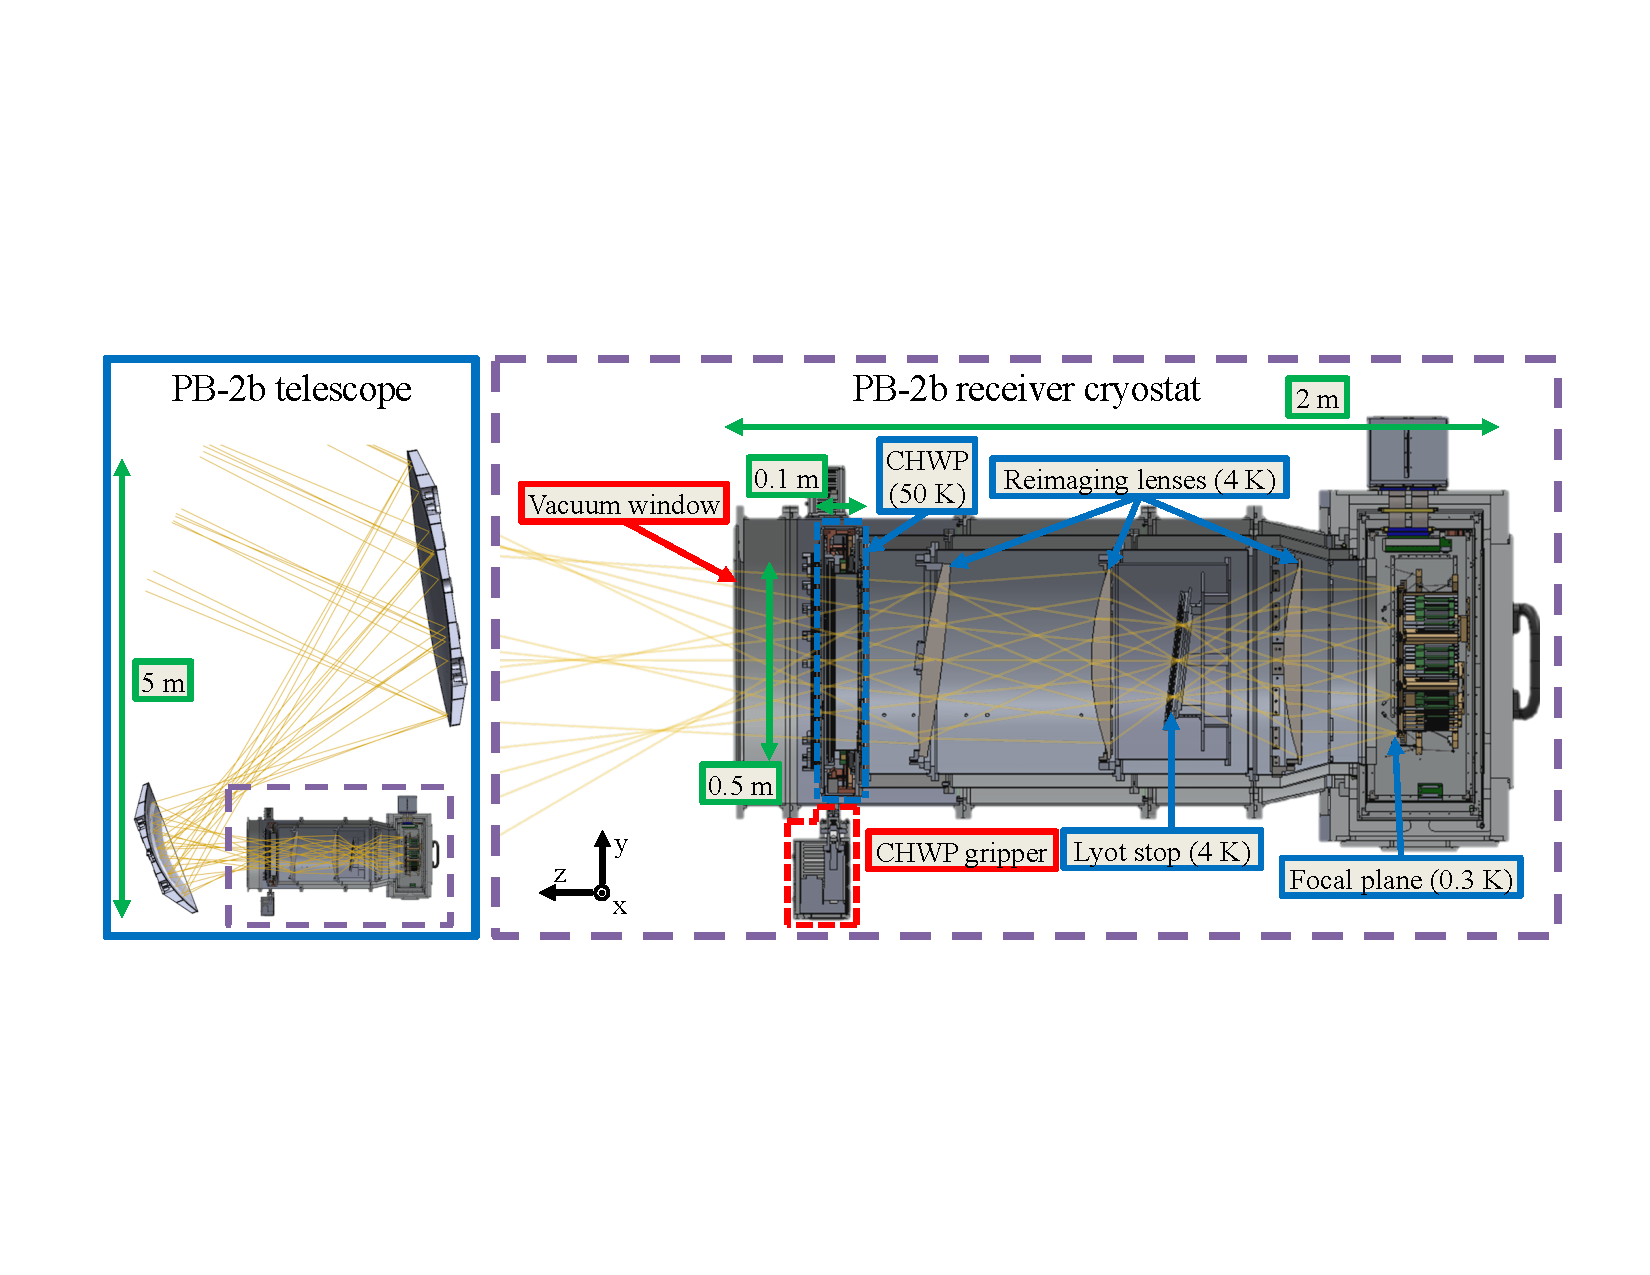
\includegraphics[width=0.98\linewidth, trim=1.5cm 5.5cm 1.5cm 5.5cm, clip]{CHWPDesign/Figures/PB2b_optical_CAD.pdf}}
    \label{fig:pb2_ray_trace}
    \subfloat[\label{fig:pb2b_chwp_in_ot_cad:b}]{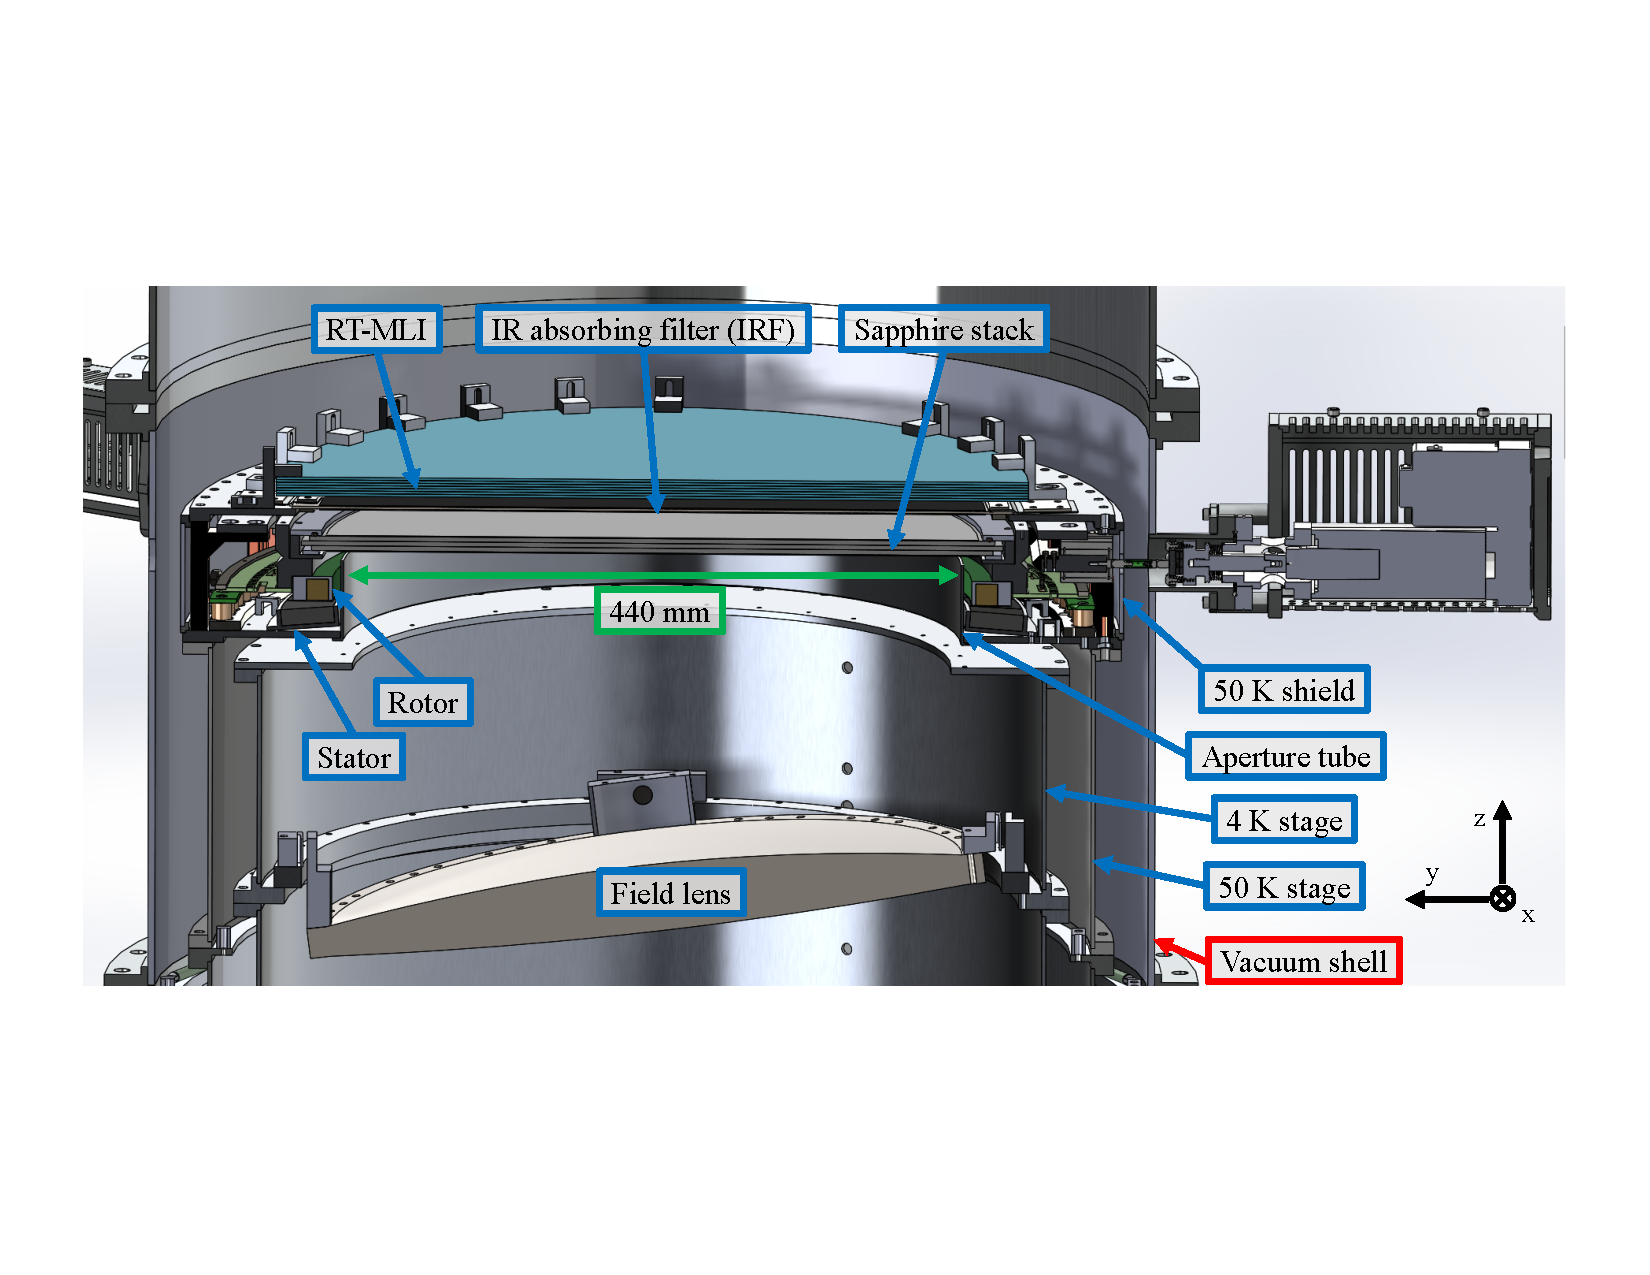
\includegraphics[width=0.98\linewidth, trim=1.5cm 4.7cm 1.5cm 5cm, clip]{CHWPDesign/Figures/CHWP_in_PB2b_CAD_crossSection.pdf}}
    \caption[CAD of the CHWP in PB-2b]{Figure~\ref{fig:pb2b_chwp_in_ot_cad:a} shows an optical ray trace of the PB-2b telescope (left) and receiver cryostat (right), superposed onto computer-aided-design (CAD) cross-sectional views. Red boxes mark warm components, and blue boxes mark cold components. The CHWP is located between the secondary mirror and the field lens and has a 440~mm clear aperture diameter. Figure~\ref{fig:pb2b_chwp_in_ot_cad:b} shows a zoomed CAD cross section of the CHWP integrated into the PB-2b optics tube, highlighting CHWP-relevant optical and thermal components. Red boxes mark warm parts, and blue boxes mark cold parts. The CHWP's clear aperture is defined by a stationary, HR-10-lined aperture tube (absorber not shown) that hides non-optical rotating components from the telescope's beam.}
    \label{fig:pb2b_chwp_in_ot_cad}
\end{figure}

In a similar way to with the PB-2a warm HWP discussion, it is useful to understand the context that surrounds the PB-2b polarization modulator. PB-2b was conceived along with Simons Array (SA), which was funded in 2015 to build three POLARBEAR-2 (PB-2) telescopes. At this point, PB-2---which was originally funded in 2012 and was being built in Japan---became PB-2a, and PB-2b and PB-2c were born. PB-2b shares many common characteristics with PB-2a, including an identical telescope, a nearly identical receiver cryostat design, alumina reimaging optics, lenslet-coupled sinuous antennas, and transition-edge sensor (TES) bolometers. However, there are a few areas where PB-2b has strove to improve, including upgraded lens coatings, improved detector wafers and readout, and using a CHWP. The PB-2b backend---which contains the focal plane infrastructure---was built at the University of California, San Diego (UCSD), while the optics tube was built at UC Berkeley. Motivated in part by its being a brand new component, the CHWP was developed at Lawrence Berkeley National Laboratory (LBNL) under the purview of Staff Scientist Akito Kusaka. CHWP R\&D launched in late 2014, the PB-2b CHWP was built and tested in 2016-2017, and it was integrated into the PB-2b optics tube in 2018. The optics tube was then moved to UCSD in 2019, where the CHWP was tested with the full receiver system, and PB-2b was deployed to Chile in early 2020. Chilean work is currently halted by the COVID-19 pandemic, but the CHWP is expected to see first light in early 2021. Therefore, the presented research the result of nearly six years of design, construction, and testing and includes several advancements in the research area of polarization modulators for CMB polarimetry.

%%%%%%%%%%%%%%%%%%%%%%%%%%%%%%%%
%%%%%%%%%%%%%%%%%%%%%%%%%%%%%%%%
%%%%%%%%%%%%%%%%%%%%%%%%%%%%%%%%

\section{Precedent}
\label{sec:chwp_design_precedent}

Cryogenic HWPs have been deployed in several experiments before SA, and the PB-2b design leverages much of this preceding work in its own design. In particular, the PB-2b CHWP relies most notably on many aspects of the E and B EXperiment's (EBEX) continuously rotating CHWP, and therefore we want to briefly discuss this precedent before getting into the details of the PB-2b design.

EBEX was a balloon experiment that flew for 20 days above Antarctica in 2013 and observed at 150, 250, and~410~GHz. They used a five-stack AHWP and a three-layer AR coating to accommodate their tri-chroic, broadband receiver design. The EBEX CHWP was located on the 4~K stage just in front of the aperture stop, rotates on a superconducting magnetic bearing (SMB), is driven by an external motor coupled to a Kevlar belt, and is monitored by a slot-chopped angular encoder. While the EBEX flight did not achieve its scientific targets due to problems during flight, the CHWP successfully rotated 584,000 times at the nominal 1.235~Hz rotation speed and achieved a rotational velocity stability of 0.45\% per ten hour observation set. In this way, the EBEX CHWP was a success that the PB-2b CHWP design work was able to build upon for its own design. Tomotake Matsumura, who is now involved in the LiteBIRD HWP development at the Kavli Institute for the Physics and Mathematics of the Universe (Kavli IPMU), pioneered the cryogenic continuous HWP for EBEX and was also part of the early design phases of the PB-2b CHWP.

There are a few elements to the PB-2b CHWP implementation that are substantially different from those of EBEX. First, the PB-2b CHWP is located on the 50~K stage, which relaxes its power dissipation requirements. Second, it is not located at the aperture stop, which means that the beams from detectors across the focal plane are only partially overlapping, hence heightening the importance of optical-stack uniformity to suppress HWP synchronous signals (HWPSSs). Third, the PB-2b CHWP must undergo $>$~100,000,000 revolutions as opposed to 100,000, which incites a different regime of durability. And last, SA is a more powerful instrument than EBEX, and therefore systematic effects from the PB-2b CHWP must be more tightly controlled to avoid substantially degrading data quality. For these reasons, among others, many aspects of the the PB-2b CHWP design are fresh and novel.

%%%%%%%%%%%%%%%%%%%%%%%%%%%%%%%%
%%%%%%%%%%%%%%%%%%%%%%%%%%%%%%%%
%%%%%%%%%%%%%%%%%%%%%%%%%%%%%%%%

\section{Requirements}
\label{sec:chwp_design_requirements}

The CHWP must meet several optical, thermal, noise, and operational requirements in order to effectively mitigate 1/f noise and I-to-P leakage while not introducing its own systematic effects. These requirements are central to the CHWP design and depend on the specifics of PB-2b's telescope, cryogenic, and detector systems. 

When it was conceived, PB-2b was virtually a copy of PB-2a \cite{matsumura_polarbear-2_2012}, which does not use a CHWP. As a result, the CHWP is retrofitted to the original PB-2b design and centers around maintaining ``heritage'' system performance. Table~\ref{tab:requirements} summarizes the PB-2b CHWP's numerical requirements and achieved values. In the following subsections, we detail the CHWP's design drivers and how they flow into its hardware specifications. 

\begin{table}
\caption{The CHWP's numerical requirements and achieved values.}
\label{tab:requirements}
\centering
\begin{tabu}{|l|l|l|}
\hline
\textbf{Parameter} & \textbf{Requirement} & \textbf{Achieved} \\
\hline
\hline
Assembly outer diameter & $\leq$ 700~mm & 690~mm \\
\hline
Assembly height & $\leq$ 100~mm & 95~mm \\
\hline
Clear aperture diameter & $\geq$ 430~mm & 440~mm \\
\hline
Rotor temperature $T_{\mathrm{rotor}}$ & $\leq$ 55~K & $<$~53~K \\
\hline
Thermal dissipation $P_{\mathrm{stator}}$ & $\leq$ 2~W & $<$~1.3 W \\
\hline
Rotor thermalization time & $\leq$ 36~hr & 5~hr \\
\hline
Rotation frequency $f_{\mathrm{HWP}}$ & $\geq$ 2~Hz & $\leq$ 2.8~Hz \\
\hline
Angle encoder noise $\sigma_{\chi}$ & $\ll$ 3 $\mathrm{\mu rad / \sqrt{Hz}}$ & 0.1~$\mathrm{\mu rad / \sqrt{Hz}}$ \\
\hline
B-field interference $\sigma_{\mathrm{B}}$ @ 4$f_{\mathrm{HWP}}$ & $\ll$~20~$\mathrm{\mu G / \sqrt{Hz}}$ & $<$~10~$\mathrm{\mu G / \sqrt{Hz}}$\\
\hline
$T_{\mathrm{rotor}}$ stability $\sigma_{T_{\mathrm{rotor}}}$ @ 1~mHz & $\ll$ 1~$\mathrm{mK / \sqrt{Hz}}$ & $<$~0.3~$\mathrm{mK / \sqrt{Hz}}$ \\
\hline
\end{tabu}
\end{table}

%%%%%%%%%%%%%%%%%%%%%%%%%%%%%%%%
%%%%%%%%%%%%%%%%%%%%%%%%%%%%%%%%

\subsection{Spatial and optical requirements}
\label{sec:spatial_requirements}

The initial set of requirements are on the CHWP's physical dimensions. As shown in Figure~\ref{fig:pb2b_chwp_in_ot_cad}, the assembly must fit within the confines of the optics tube's vacuum shell, limiting its cryogenic diameter to $\leq$~700~mm. Additionally, its height, or dimension along the z-axis, must be $\leq$~100~mm so that the window aperture does not extend too far toward the secondary mirror, where the telescope's beam\footnote{The telescope's beam is defined to be the collection of reverse-time-sense rays from all detectors on the focal plane.} diverges more rapidly than within the receiver. These dimensional constraints influence much of how the CHWP subsystems are built and arranged, as well as their clearances and alignment tolerances.

\begin{figure}[!t]
    \centering
    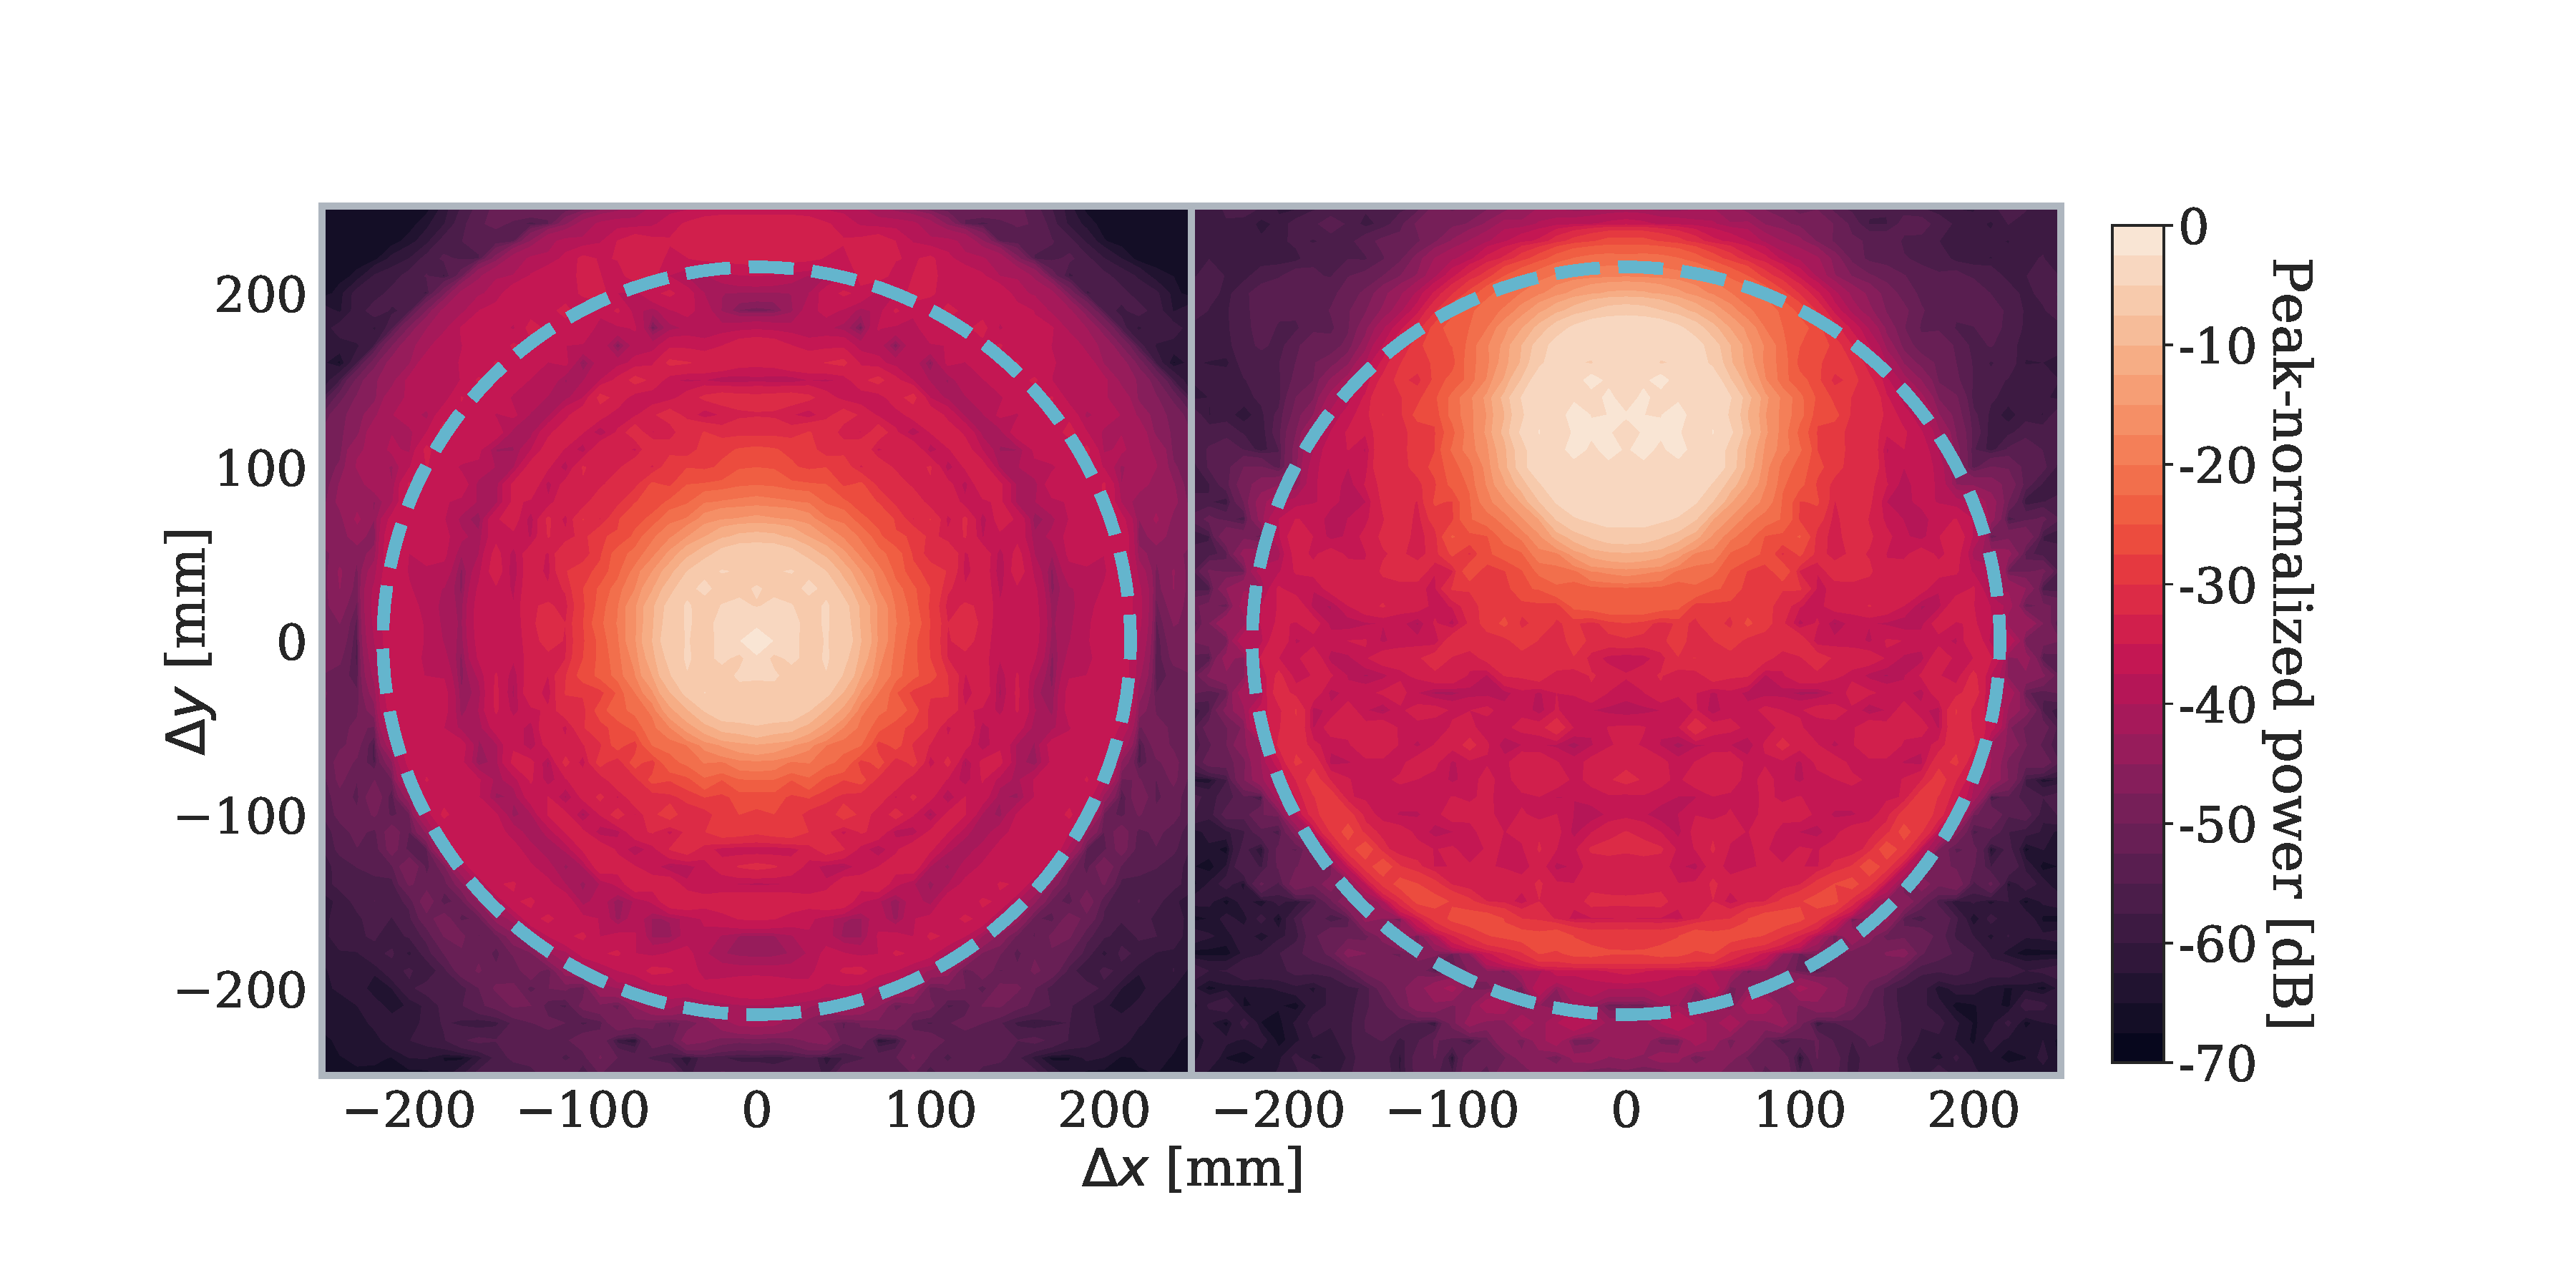
\includegraphics[width=\linewidth, trim=3cm 2cm 5cm 4cm, clip]{CHWPDesign/Figures/chwp_aperture_thesis.pdf}
    %\includegraphics[width=0.98\linewidth, trim=2.4cm 2.1cm 3cm 2.8cm, clip]{Figures/chwp_aperture.pdf}
    \caption{The reverse-time-sense, peak-normalized, 90~GHz, $x$-polarization illumination pattern onto the CHWP aperture plane from detector pixels at the center (top panel) and $-y$ edge (bottom panel) of the focal plane. The 430~mm aperture requirement is marked with a dashed cyan circle about the telescope's chief ray, and the total spillover for the center (edge) pixel is 0.2\% (0.1\%).}
    \label{fig:chwp_aperture}
\end{figure}

While a presentation of sapphire-stack requirements is relegated to Chapters~\ref{ch:hwp_polarization_modulation} and~\ref{ch:sapphire_ar_coating}, we do discuss the clear aperture diameter, which is central to the cryo-mechanical design. The CHWP is located sky-side of the field lens (see Figure~\ref{fig:pb2b_chwp_in_ot_cad:a}), and its clear aperture must be large enough to admit the beam between the secondary mirror and the Gregorian focus. We use GRASP\footnote{GRASP: https://www.ticra.com/software/grasp/} to simulate the polarized, 90~GHz response of detector pixels across the focal plane, and Figure~\ref{fig:chwp_aperture} shows the $x$-polarization illumination of the central and $-y$ edge pixels at the CHWP aperture. To set a requirement, we vary the CHWP aperture diameter and compare the telescope's far-field beam to that with the CHWP aperture removed. We evaluate a collection of merit figures, including angular resolution, spill over the primary mirror, side-lobe amplitude, and differential pointing and ellipticity \cite{shimon_cmb_2008}. We find that a 430~mm aperture has no impact on the central pixel and has edge-pixel impacts that are subdominant to preexisting systematic effects in the telescope optics. Therefore, we require that the CHWP aperture encapsulate a 430~mm diameter circle about the telescope's chief ray, including a margin for manufacturing and alignment tolerances.

Additionally, we require all rotating, non-optical CHWP components to be hidden from the beam in order to minimize rotation-synchronous signals. To satisfy this requirement, the bearing and sapphire must be sufficiently oversized to encapsulate the optical baffling that defines the CHWP aperture, as shown in Figure~\ref{fig:pb2b_chwp_in_ot_cad:b}. 

%%%%%%%%%%%%%%%%%%%%%%%%%%%%%%%%
%%%%%%%%%%%%%%%%%%%%%%%%%%%%%%%%

\subsection{Thermal requirements}
\label{sec:thermal_requirements}

The next set of requirements are on the CHWP's thermal impact. Because the PB-2b detectors are expected to be photon-noise limited, CHWP-induced optical power can dramatically degrade experiment sensitivity. Figure~\ref{fig:mapping_speed} shows the simulated \cite{hill_bolocalc_2018} fractional impact of rotor temperature on PB-2b mapping speed, compared to that of a PB-2a-style warm HWP (WHWP) \cite{hill_design_2016}. Mapping speed (see Section~\ref{sec:N_ell_mapping_speed}) quantifies the number of detector-hours needed to reach a specified CMB map depth, and therefore fractional mapping speed is analogous to detector yield or observation efficiency. In this simulation, the CHWP is assumed to have an epoxy-based anti-reflection (AR) coating \cite{rosen_epoxy-based_2013}, and sensitivity degradation with increasing CHWP temperature is primarily due to increasing mm-wave emission, which in turn increases detected photon noise. As shown by the WHWP points, some of the sensitivity loss at $\approx$~270~K can be reclaimed by optimizing the AR coating for lower ambient emissivity, but the biggest sensitivity gain comes from cooling the HWP to cryogenic temperatures. Mapping speed retention is $>$~97\% when the CHWP is at $<$~50~K, and the sensitivity loss vs. CHWP temperature is gentle <~100~K. Therefore, the dominant driver of the rotor's temperature is not the CHWP's mm-wave emission but instead its IR emission onto the field lens. 

In the heritage PB-2b design without the CHWP, the 4~K field lens is radiatively loaded by the IRF (see Figure~\ref{fig:pb2b_chwp_in_ot_cad:b}). Therefore, if the CHWP becomes warmer than the IRF or if its dissipation onto the 50~K stage is too large, the CHWP-induced 4~K load will exceed that of the heritage configuration, which may in turn increase lens and Lyot temperatures and even degrade the performance of the sub-kelvin stage. Section~\ref{sec:thermal_design} discusses the CHWP thermal system in detail, and Figure~\ref{fig:rotor_temp} shows the relationship between rotor temperature and field-lens load. We require that the 4~K load not exceed that of the heritage configuration at 85\% confidence, in turn requiring the rotor temperature to be
\begin{equation}
    T_{\mathrm{rotor}} \leq 55 \; \mathrm{K} \, .
    \label{eq:rotor_temp}
\end{equation}

\begin{figure}[!t]
    \centering
    \subfloat[\label{fig:chwp_mapping_speed:a}]{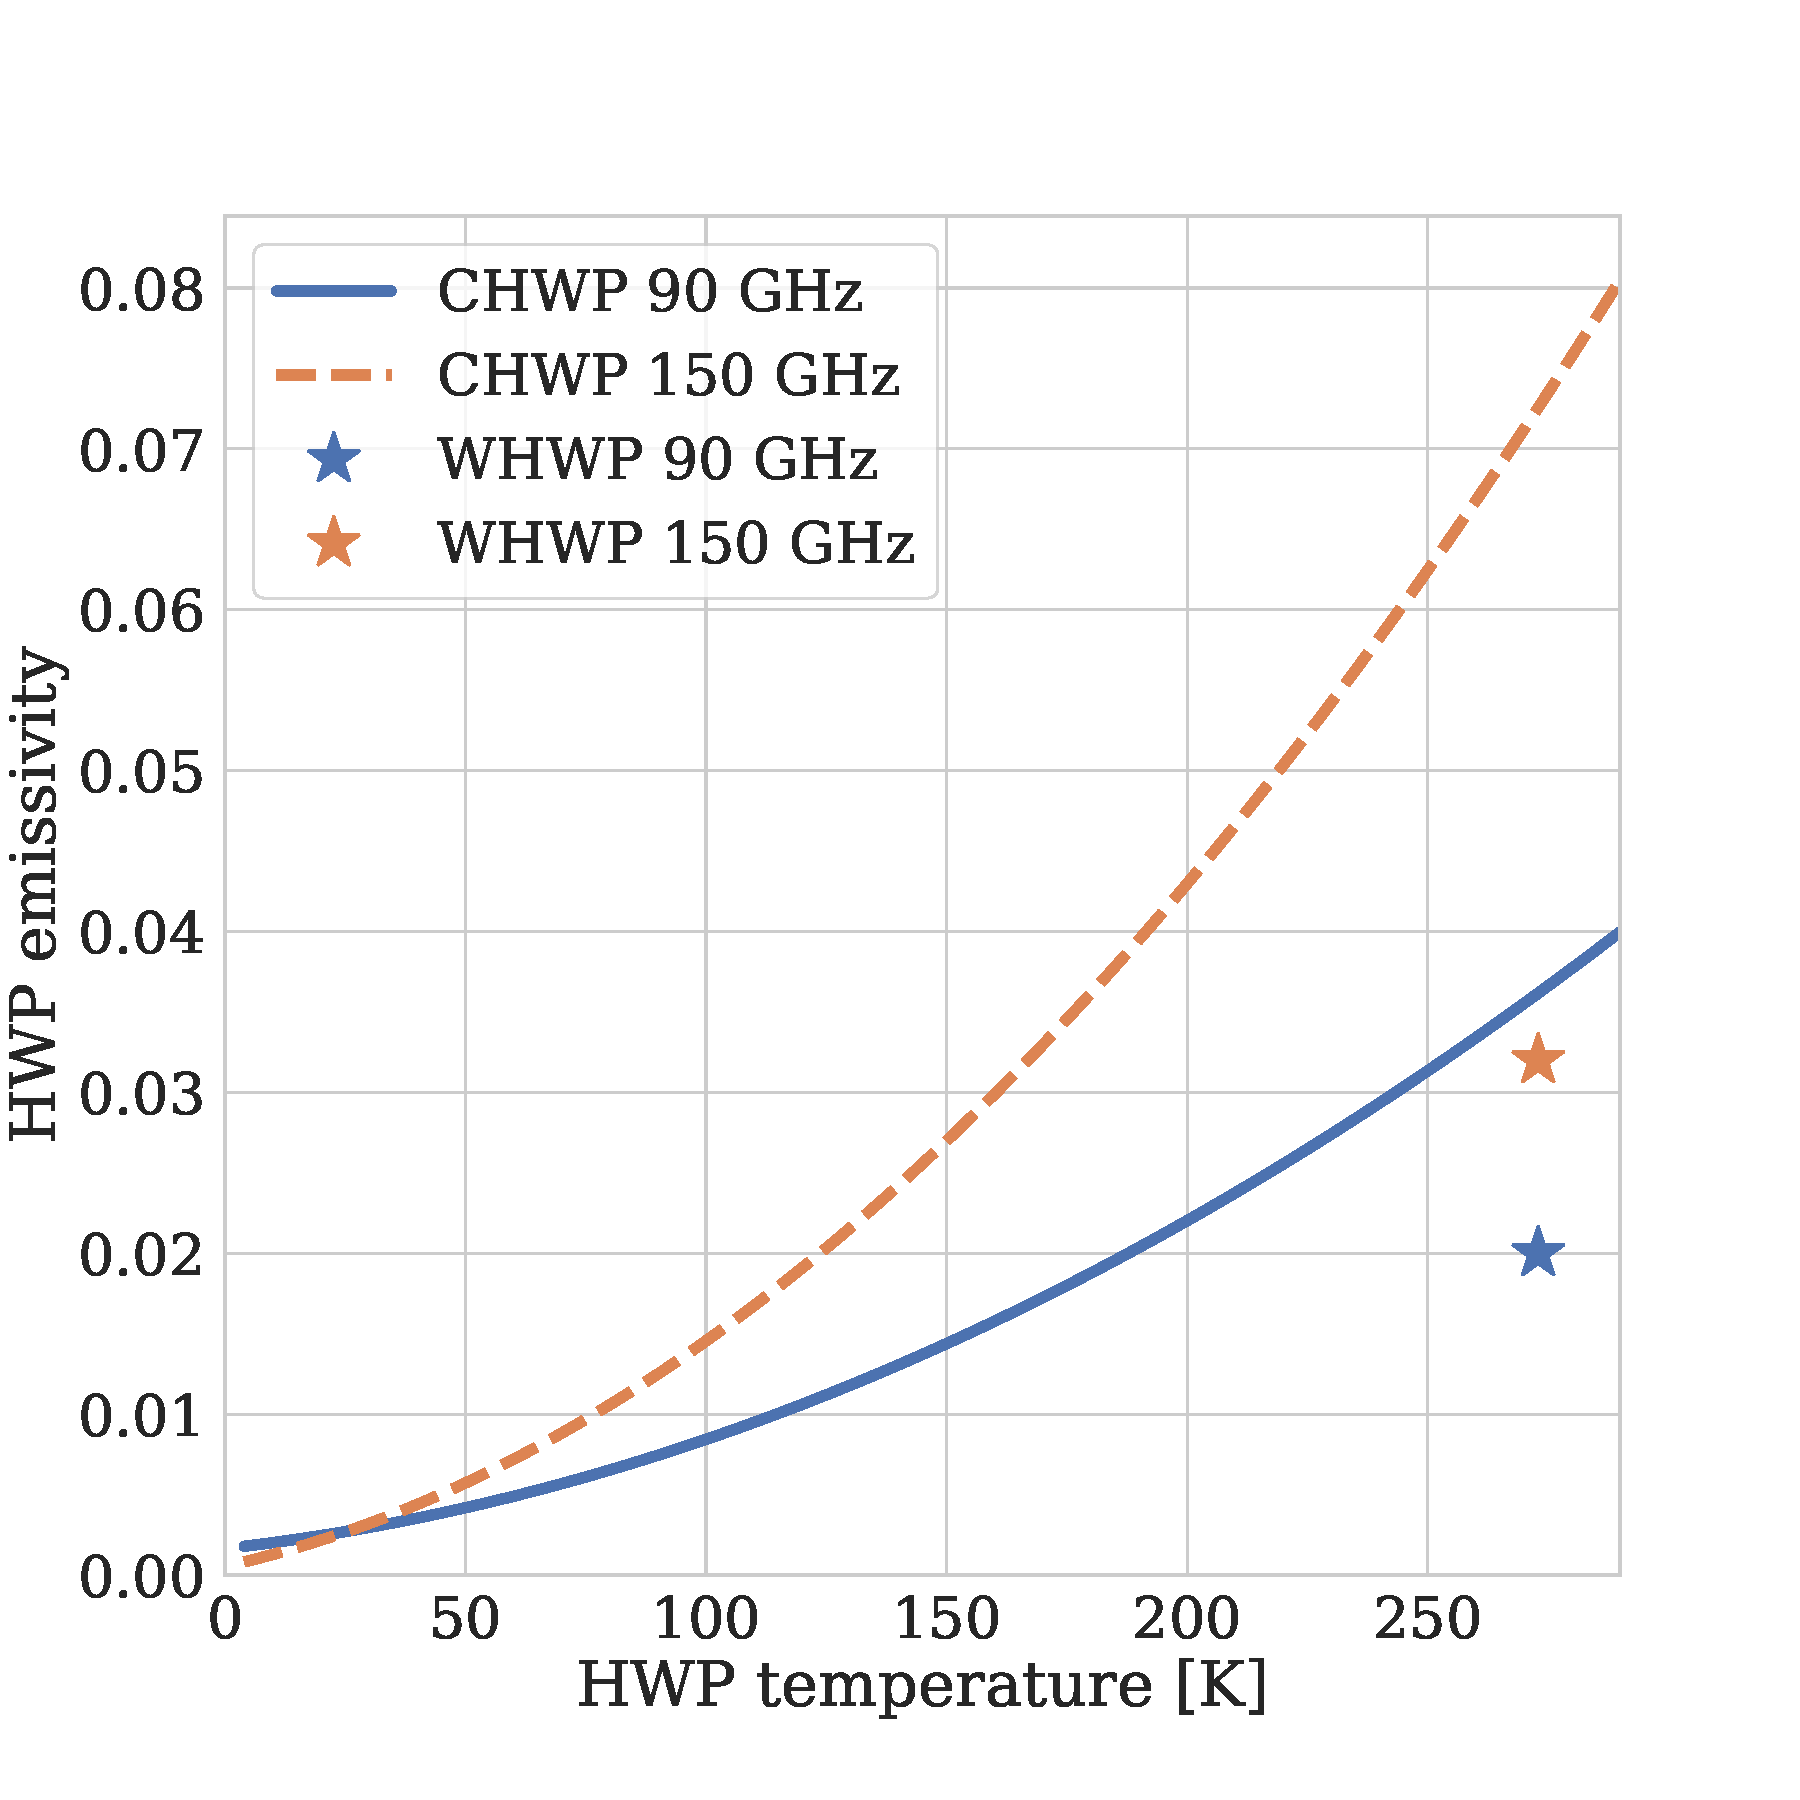
\includegraphics[width=0.5\linewidth, trim=0cm 1cm 2.5cm 3cm, clip]{CHWPDesign/Figures/hwpEmissivity_vs_hwpTemp.pdf}}
    \subfloat[\label{fig:chwp_mapping_speed:b}]{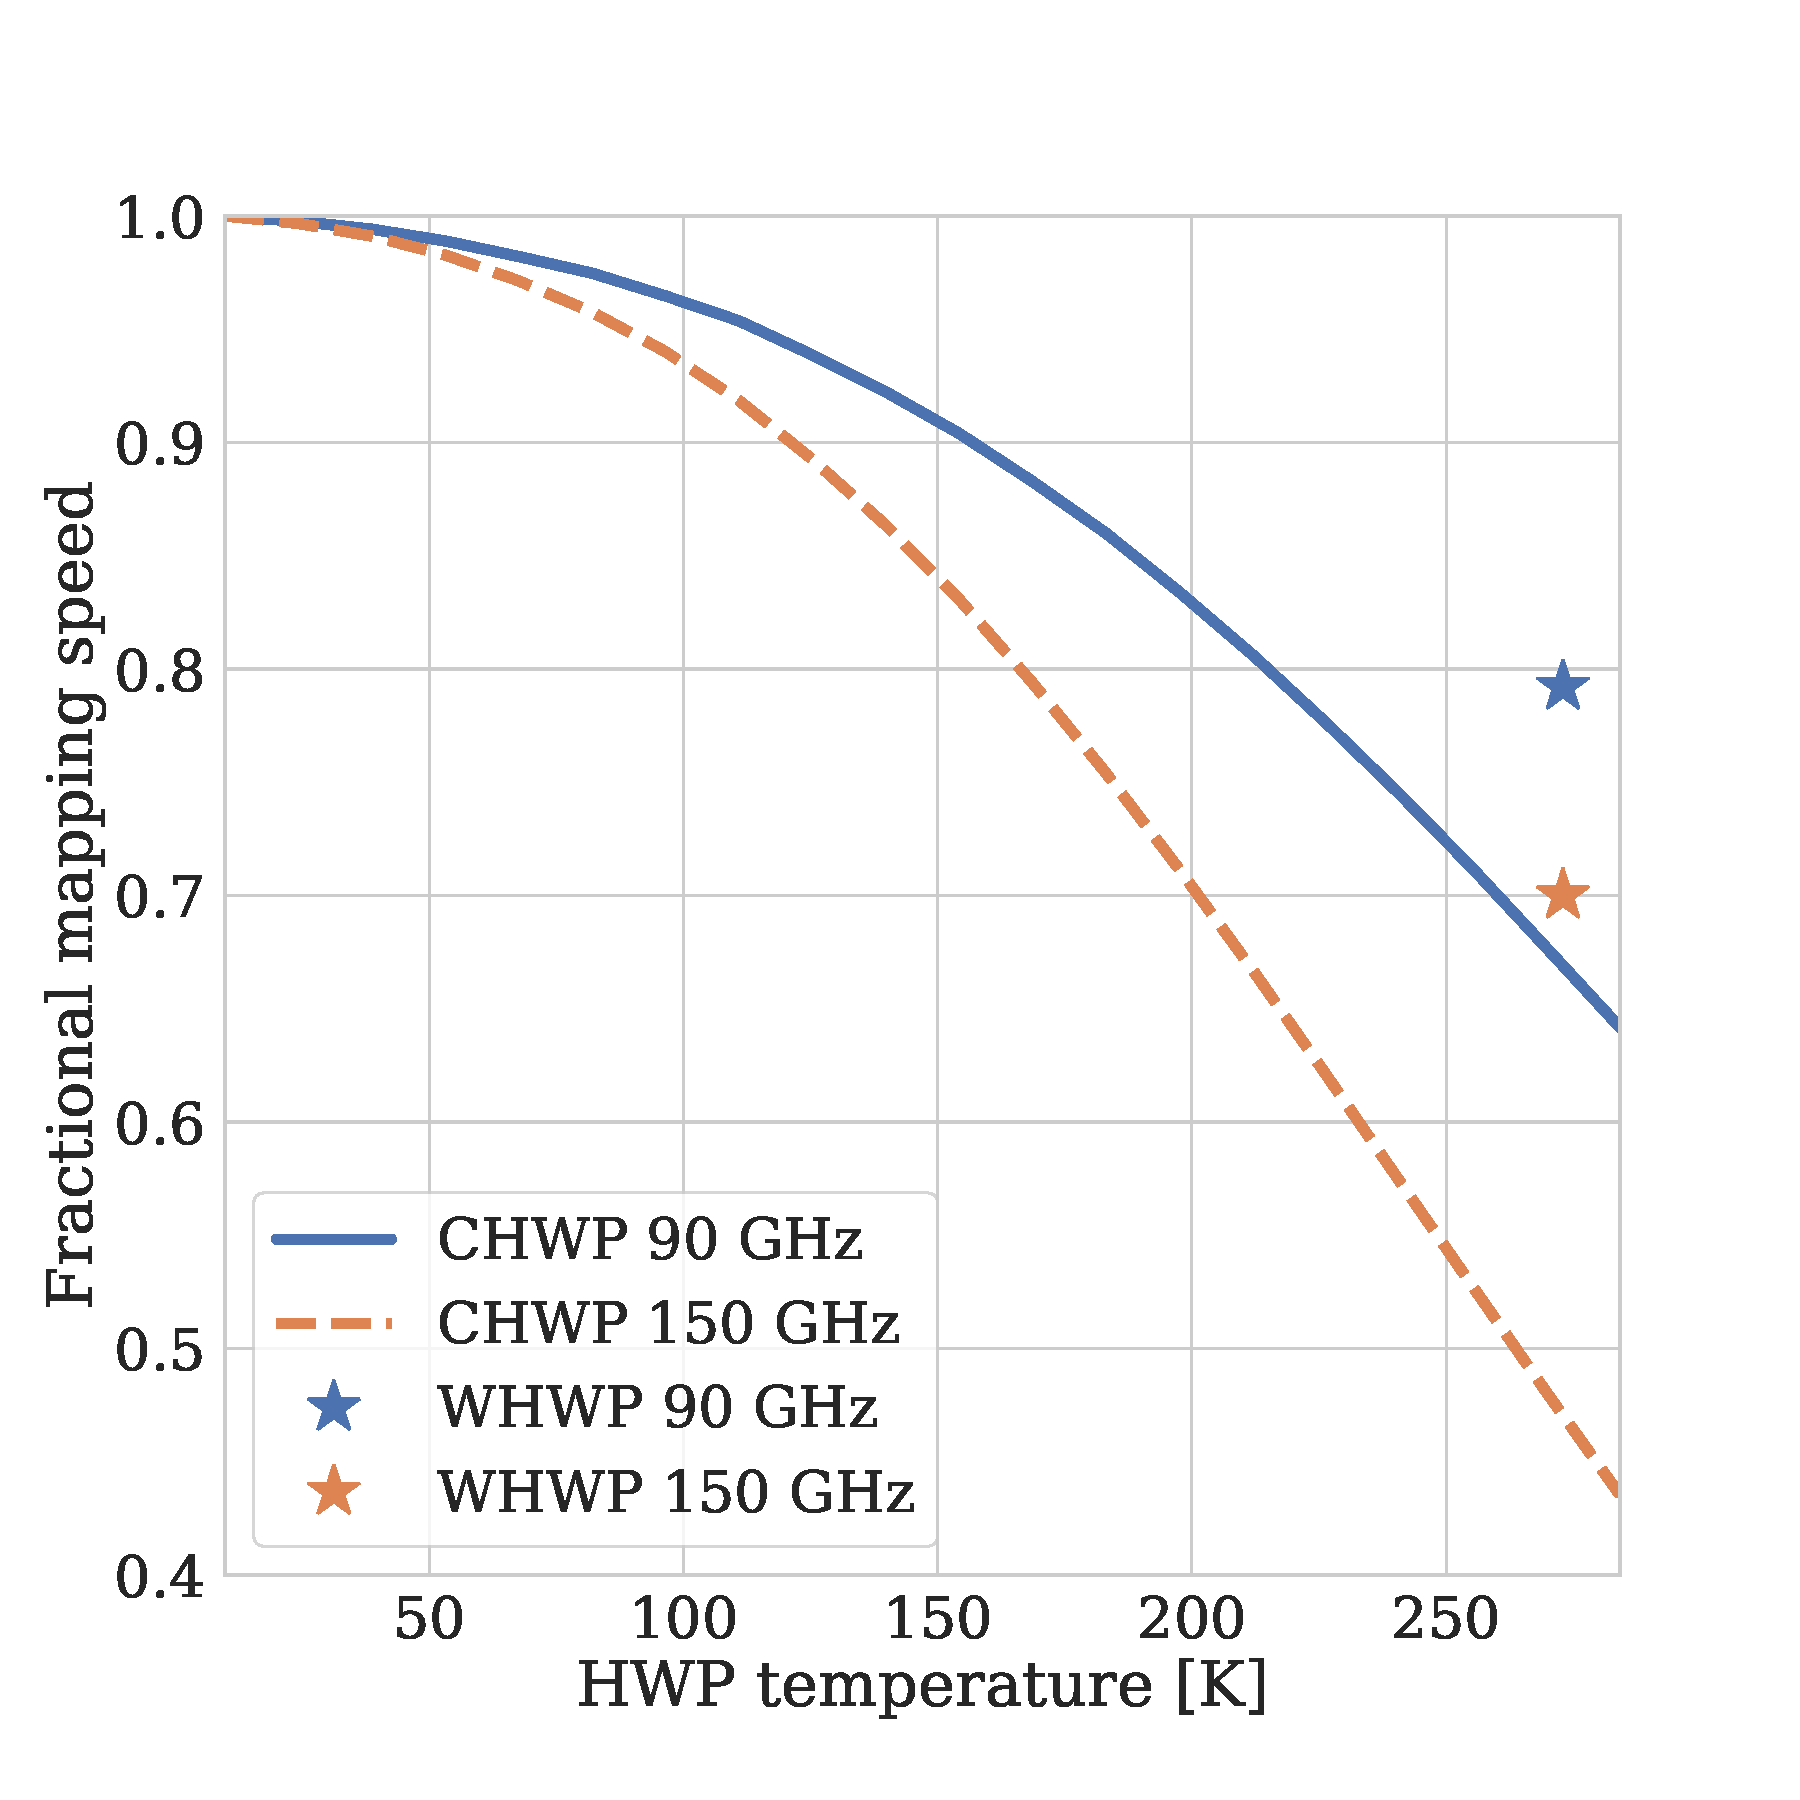
\includegraphics[width=0.5\linewidth, trim=-0.5cm 1cm 3cm 3cm, clip]{CHWPDesign/Figures/HWP_fractionalMappingSpeed.pdf}}
    \caption{The fractional impact of rotor temperature on PB-2b mapping speed with respect to that of a 4~K HWP, compared to that of a PB-2a-style warm HWP (WHWP) at 273~K.\cite{hill_design_2016} Note that the mapping speed gain of a 4~K CHWP over a 50~K CHWP is $\approx$ 1\%.}
\label{fig:mapping_speed} 
\end{figure}

It is unavoidable that dissipation from the CHWP motor and bearing will warm the 50~K stage, raising IRF and rotor temperatures. The goal, however, is to keep this temperature rise small enough to not warm 4~K components. Utilizing load-curve measurements of the PB-2b optics tube,\cite{howe_polarbear-2_2019} we mandate that the CHWP warm the 50~K stage $<$~1~K with respect to the heritage configuration and therefore set the CHWP's 50~K dissipation requirement to be
\begin{equation}
    P_{\mathrm{stator}} \leq 2 \; \mathrm{W} \, .
    \label{eq:stator_power}
\end{equation}

We next require that the CHWP not add to the PB-2b cooldown time. This mandate is important both for restarting observations following a disruption in the field and for rapid-turnaround receiver testing in the lab. The heritage PB-2b system takes about five days to cool, and that duration is limited by the cooldown of the focal plane, which reaches 4~K about 36~hours after the optics tube \cite{howe_polarbear-2_2019}. The CHWP's cooldown time is limited by that of the rotor, which has a large thermal mass and is heatsinked by unfastened interfaces (see Section~\ref{sec:gripper_design}). Therefore, we require that the rotor reach its base temperature before the focal plane has thermalized, or within 36~hours of the 50~K stage.

Finally, we require that CHWP operation not vibrate the focal plane structure. CHWP-induced vibrations can generate microphonic heating that may modulate the focal plane's temperature and degrade detector gain stability \cite{howe_polarbear-2_2019}. To avoid such issues, we require no measurable difference in focal-plane temperature between when the rotor is spinning and when it is not.

%%%%%%%%%%%%%%%%%%%%%%%%%%%%%%%%
%%%%%%%%%%%%%%%%%%%%%%%%%%%%%%%%

\subsection{Noise requirements}
\label{sec:noise_requirements}

In order for the CHWP to effectively suppress 1/f noise, $f_{\mathrm{m}} = 4 f_{\mathrm{HWP}}$ must be large enough such that all modulation sidebands, which are contained within $4 f_{\mathrm{HWP}} \pm \Delta f$, are above the Atacama's 1$\sim$2~Hz knee frequency \cite{takakura_performance_2017,kusaka_modulation_2014}, or the frequency at which 1/f noise power and white noise power are equal. Assuming a $0.4^{\circ}$/s telescope scan speed \cite{the_polarbear_collaboration_measurement_2020}, the sky is fully resolved by $\approx$~4~Hz of temporal bandwidth \cite{takakura_performance_2017}. Therefore, we require
\begin{equation}
    f_{\mathrm{HWP}} \geq 2 \; \mathrm{Hz}
    \label{eq:rot_freq_requirement} \, ,
\end{equation}
\noindent
which places the demodulation band $4f_{\mathrm{HWP}} \pm \Delta f = 8 \pm 4$~Hz comfortably clear of atmospheric fluctuations. PB-1 and the Atacama B-mode Search (ABS) also rotate their HWPs at $\approx$~2~Hz in Chile and achieve excellent 1/f suppression in their demodulated detector data \cite{takakura_performance_2017,kusaka_modulation_2014}.

While rejecting optical 1/f noise, the CHWP introduces other noise sources that can degrade data quality. These CHWP-induced noise sources are largely common-mode across the focal plane and hence do not average down during detector coaddition. Therefore, we require the noise equivalent CMB temperature ($\mathrm{NET_{CMB}}$) of each CHWP noise source to be much less than the forecasted PB-2b array-averaged $\mathrm{NET_{CMB}}$ \cite{suzuki_polarbear-2_2016}
\begin{equation}
    \mathrm{NET_{CMB}^{HWP}} \ll \mathrm{NET_{CMB}^{arr}} = 5.8 \; \mathrm{\mu K_{CMB} / \sqrt{Hz}} \, .
    \label{eq:arr_noise}
\end{equation}
\noindent
We use this bound to set requirements on three primary CHWP contaminants: encoder angle jitter, magnetic interference, and rotor temperature stability.

Firstly, encoder angle noise injects noise into the demodulated detector data. The CHWP is located behind the telescope's off-axis mirrors, which induce I-to-P along the $y$ direction (see Figure~\ref{fig:pb2b_chwp_in_ot_cad:a}). This I-to-P is modulated at 4$f_{\mathrm{HWP}}$, and an imperfect rotor angle measurement will imperfectly subtract the telescope signal during demodulation. PB-1 measures up to $\approx$~180~$\mathrm{mK_{\mathrm{RJ}}}$ of I-to-P at the prime focus of an SA-style telescope, largely due to emission from the primary reflector \cite{takakura_performance_2017}. Because the PB-2b CHWP is located behind the primary \textit{and} secondary mirrors, we conservatively\footnote{In reality, we expect the I-to-P from the secondary reflector to be less than that of the primary due to its being ellipsoidal with a smaller incident angle. However, the secondary mirror's emission has not been studied in detail, and so we assert that each mirror generates similar I-to-P leakage in order to set a conservative angle jitter requirement.} assert an I-to-P amplitude of
\begin{equation}
    A_{4}^{0} \sim 400 \; \mathrm{mK_{\mathrm{RJ}}} \, .
    \label{eq:4f_amp}
\end{equation}
\noindent
This mirror polarization is modulated at 4$f_{\mathrm{HWP}}$, and a mismeasurement $\Delta \chi$ of the CHWP angle $\chi$ modifies the 4$f_{\mathrm{HWP}}$ amplitude $A_{4}(\chi)$ as
\begin{eqnarray}
    A_{4}(\chi) &&= A_{4}^{0} \mathrm{cos}(4 \left[ \chi + \Delta \chi \right] ) \nonumber \\ &&\approx A_{4}^{0} \mathrm{cos}(4 \chi) - 4 \, A_{4}^{0} \mathrm{sin}(4 \chi) \Delta \chi \, ,
    \label{eq:freq_mod}
\end{eqnarray}
\noindent
such that
\begin{equation}
    \Delta A_{4} = -4 \, A_{4}^{0} \mathrm{sin}(4 \chi) \Delta \chi \, .
    \label{eq:delta_chi}
\end{equation}
Assuming that the angle jitter is random, its average effect on the detected noise spectrum is
\begin{equation}
    \mathrm{NET_{CMB}^{HWP}} = 2 \sqrt{2} \,  \frac{\mathrm{d} T_{\mathrm{CMB}}}{\mathrm{d} T_{\mathrm{RJ}}} \, A_{4}^{0} \, \sigma_{\chi} \, ,
    \label{eq:encoder_noise}
\end{equation}
\noindent
where $\sigma_{\chi}$ is the root mean square (RMS) of $\Delta \chi$ and $\mathrm{d} T_{\mathrm{CMB}} / \mathrm{d} T_{\mathrm{RJ}} = 1.7$ is evaluated at 150~GHz. Mandating that $\mathrm{NET_{CMB}^{HWP}} \ll \mathrm{NET_{CMB}^{arr}}$ (see Equation~\ref{eq:arr_noise}), the angle noise requirement is
\begin{equation}
    \sigma_{\chi} \ll 3 \, \mathrm{\mu rad / \sqrt{Hz}} \, .
\end{equation}

Secondly, CHWP-induced magnetic interference can also inject noise into the demodulated data. The PB-2b detector array consists of aluminum manganese (AlMn) transition-edge sensors (TESs) amplified by superconducting quantum interference devices (SQUIDs). Both AlMn TESs and SQUIDs are sensitive to ambient magnetic fields, and because the PB-2b CHWP consists of a magnetic bearing and an electromagnetic motor (see Sec.~\ref{sec:chwp_design}), magnetic interference at the focal plane must be carefully controlled.

PB-2b uses gradiometric Series SQUID Array Amplifiers (SSAAs) \cite{stiehl_time-division_2011} fed back using Digital Active Nulling \cite{haan_improved_2012}, stabilized by a low-frequency flux-locked loop \cite{Bender2014}, and shielded via a combination of $\mu$-metal and superconducting niobium \cite{xu_combined_1987}.  This particular SQUID configuration is robust to time-varying magnetic fields, especially those which are uniform over each SQUID's $\sim$~10~$\mathrm{mm^{2}}$ area. Therefore, the more considerable CHWP-specific concern is magnetic interference in the detectors themselves.\footnote{Private communication with Prof. Tijmen de Haan (KEK High Energy Research Organization) and Prof. Darcy Barron (University of New Mexico), May 2020.}

Magnetic pickup at 4$f_{\mathrm{HWP}}$ mimics modulated sky polarization, especially if the magnetic signal drifts over the course of an observation. The superconducting transition temperature $T_{\mathrm{c}}$ of AlMn varies slightly with ambient magnetic field $B$ \cite{deiker_superconducting_2004}, and a change in $T_{\mathrm{c}}$ changes the bolometer's saturation power $P_{\mathrm{sat}}$, which in turn mimics a change in optical power $P_{\mathrm{opt}}$. We can convert the CHWP-induced magnetic jitter $\sigma_{\mathrm{B}}$ to $\mathrm{NET_{CMB}}$ as
\begin{equation}
    \mathrm{NET_{CMB}^{HWP}} = \frac{\mathrm{d} T_{\mathrm{CMB}}}{\mathrm{d} P_{\mathrm{opt}}} \frac{\mathrm{d} P_{\mathrm{sat}}}{\mathrm{d} T_{\mathrm{c}}} \frac{\mathrm{d} T_{\mathrm{c}}}{\mathrm{d} B} \sigma_{B} \, .
    \label{eq:pbias_bfield}
\end{equation}
\noindent
Measurements of the PB-2b AlMn TESs give $\mathrm{d} T_{\mathrm{c}} / \mathrm{d} B = 0.3$~mK/G \cite{vavagiakis_magnetic_2018} and $\mathrm{d} P_{\mathrm{sat}} / \mathrm{d} T_{\mathrm{c}} = 0.1$~pW/mK \cite{westbrook_polarbear-2_2018}, while simulations of the PB-2b optics \cite{hill_bolocalc_2018} give $\mathrm{d} T_{\mathrm{CMB}} / \mathrm{d} P_{\mathrm{opt}} = 12$~$\mathrm{\mu K_{CMB} / aW}$. We again require that $\mathrm{NET_{CMB}^{HWP}} \ll \mathrm{NET_{CMB}^{arr}}$ such that 
\begin{equation}
    \sigma_{\mathrm{B}} \; @ \; 4f_{\mathrm{HWP}} \ll 20 \; \mathrm{\mu G / \sqrt{Hz}} \, .
    \label{eq:mag_requirement}
\end{equation}
\noindent

The final noise requirement is on the CHWP rotor temperature stability.  Thermal emission from the CHWP can be modulated at 4$f_{\mathrm{HWP}}$ due to non-uniformities in the sapphire stack \cite{salatino_studies_2018}. In turn, variations in CHWP temperature will modulate the amplitude of this thermal signal, mimicking polarized sky fluctuations in the demodulated detector data. At 50~K, the thermal 4$f_{\mathrm{HWP}}$ amplitude is expected to arise predominantly due to thickness and index variations in the AR coating, as sapphire is very transparent at mm wavelengths and low temperatures \cite{parshin_silicon_1995,braginsky_experimental_1987}. While a detailed study of AR coating uniformity is relegated to Chapter~\ref{ch:sapphire_ar_coating}, we can set an empirical limit by once again invoking the PB-1 HWP's 4$f_{\mathrm{HWP}}$ amplitude (see Equation~\ref{eq:4f_amp}), which is $\sim$~10\% of its thermal emission \cite{takakura_performance_2017}. We assume that the PB-2b CHWP's 4$f_{\mathrm{HWP}}$ thermal signal will also be 10\% of its thermal emission to set a conservative\footnote{While a substantial portion of the PB-1 4$f_{\mathrm{HWP}}$ signal is due to polarized emission from the primary mirror (as discussed earlier in Section~\ref{sec:requirements}), we assume here that it is entirely due to HWP non-uniformity in order to set a conservative requirement on CHWP temperature stability.} requirement on its temperature stability.

Rotor temperature fluctuations $\sigma_{T_{\mathrm{rotor}}}$ can be converted to $\mathrm{NET_{CMB}}$ as
\begin{equation}
     \mathrm{NET_{CMB}^{HWP}} = \frac{0.1 \epsilon}{\eta} \frac{\mathrm{d} T_{\mathrm{CMB}}}{\mathrm{d} T_{\mathrm{RJ}}} \sigma_{T_{\mathrm{rotor}}} \, ,
\end{equation}
\noindent
where $\epsilon = 0.02$ is the assumed CHWP emissivity \cite{rosen_epoxy-based_2013}, $\eta = 0.9$ is the optical efficiency of the telescope + atmosphere between the CHWP and the CMB, and $\mathrm{d} T_{\mathrm{CMB}} / \mathrm{d} T_{\mathrm{RJ}} = 1.7$ is evaluated at 150~GHz. Noting that rotor temperature fluctuations follow a 1/f spectrum, we require $\mathrm{NET_{CMB}^{HWP}} \ll \mathrm{NET_{CMB}^{arr}}$ on 1,000~s timescales---long enough to encapsulate many long-baseline telescope traversals---which imposes a rotor temperature stability requirement of 
\begin{equation}
    \sigma_{T_{\mathrm{rotor}}} \; @ \; 1 \; \mathrm{mHz} \ll 1~\mathrm{mK / \sqrt{Hz}} \, .
    \label{eq:chwp_temp_requirement}
\end{equation}

%%%%%%%%%%%%%%%%%%%%%%%%%%%%%%%%
%%%%%%%%%%%%%%%%%%%%%%%%%%%%%%%%

\subsection{Operational requirements}
\label{sec:operational_requirements}

As the only moving component inside of the receiver cryostat, the CHWP poses unique risks to experiment operations. PB-2b intends to observe for at least three years in Chile, and the CHWP must operate robustly for as long as it is needed. This situational constraint gives rise to several operational requirements, which we highlight below.

First, the CHWP must be robust against component degradation. Because warming, opening, and cooling the receiver cryostat cost weeks of observation time, the rotor should be able to undergo $>$~100,000,000 revolutions without being serviced. This robustness requirement drives many aspects of the CHWP design, such as a zero-contact drive and multiple hardware redundancies. Second, standard CHWP operation must require no human intervention. Critical monitoring data, such as encoder data packet drops, rotational velocity, temperatures, and gripper status, are automatically logged. Additionally, the CHWP control software comprises a system of classes, configuration files, and command-line executables designed to interface with the observatory control program in order to fully automate routine operations. Rotor temperature monitoring is particularly important and is discussed in Section~\ref{sec:rotor_thermometry}.

Third, we mandate an automated shutdown procedure to keep the rotor centered if site power is lost. Weather events are not uncommon on Cerro Toco and can cause sudden generator failures. If PTR cooling terminates and site network access is unavailable, the CHWP must automatically stop and stow such that it can reliably restart with minimal performance degradation. Shutdown and recovery testing was central to system evaluation and is discussed in Section~\ref{sec:pb2a_chwp_evaluation_shutdown_recovery}. Fourth, in the event of critical equipment failures, an issue with the sapphire stack, or an otherwise unforeseen problem, the CHWP must be simple to service on the telescope. This requirement motivates the CHWP's location near the vacuum window where it can be accessed with minimal disassembly, as discussed in Section~\ref{sec:assembly_procedure}.

%%%%%%%%%%%%%%%%%%%%%%%%%%%%%%%%
%%%%%%%%%%%%%%%%%%%%%%%%%%%%%%%%
%%%%%%%%%%%%%%%%%%%%%%%%%%%%%%%%

\section{Cryo-mechanical assembly}
\label{sec:chwp_design_cryo_mechanical_assembly}

Given the requirements presented in Section~\ref{sec:chwp_design_requirements}, we now discuss the design of the CHWP mechanism, shown in Figures~\ref{fig:pb2b_chwp_in_ot_cad:b} and~\ref{fig:chwp_tabletop}. The CHWP consists of a rotor, stator, motor, encoder, and gripper, all integrated into a compact assembly on the 50~K stage. The following sections detail the designs of each subsystem.

%%%%%%%%%%%%%%%%%%%%%%%%%%%%%%%%
%%%%%%%%%%%%%%%%%%%%%%%%%%%%%%%%

\subsection{Location}
\label{sec:location}

The CHWP is located on the 50~K stage, which has several advantages over possible 4~K locations, such as at the Lyot stop. First, the CHWP is skyward of all reimaging optics, mitigating the impact of Fresnel I-to-P generated at the lens surfaces. Second, at 50~K, the sapphire stack's mm-wave emission is already deeply subdominant to that of other optical elements, limiting the sensitivity gain of cooling further (see Sec.~\ref{sec:thermal_requirements}). Third, the PTR's first stage has substantially more cooling power ($\sim$~10~W/K) than its second ($\sim$~1~W/K), relaxing CHWP dissipation requirements. Fourth, the focal plane structure is anchored to the 4~K stage but not the 50~K, easing CHWP vibrational requirements. Fifth, the 50~K location necessitates minimal optics-tube assembly/disassembly to install/access the CHWP, making it easy to both integrate into the receiver and service on the telescope, if necessary. Finally, the 50~K CHWP is modular, with its addition to the PB-2b instrument requiring no adjustment to the heritage lens shapes or positions, thermal filtering, or optics tube assembly procedure. This final feature was particularly powerful for PB-2b integration and testing, allowing the CHWP and optics tube to be validated in parallel prior to full system integration, hence accelerating the receiver commissioning process.

\begin{figure}[!t]
    \centering
    \subfloat[\label{fig:chwp_tabletop:a}]{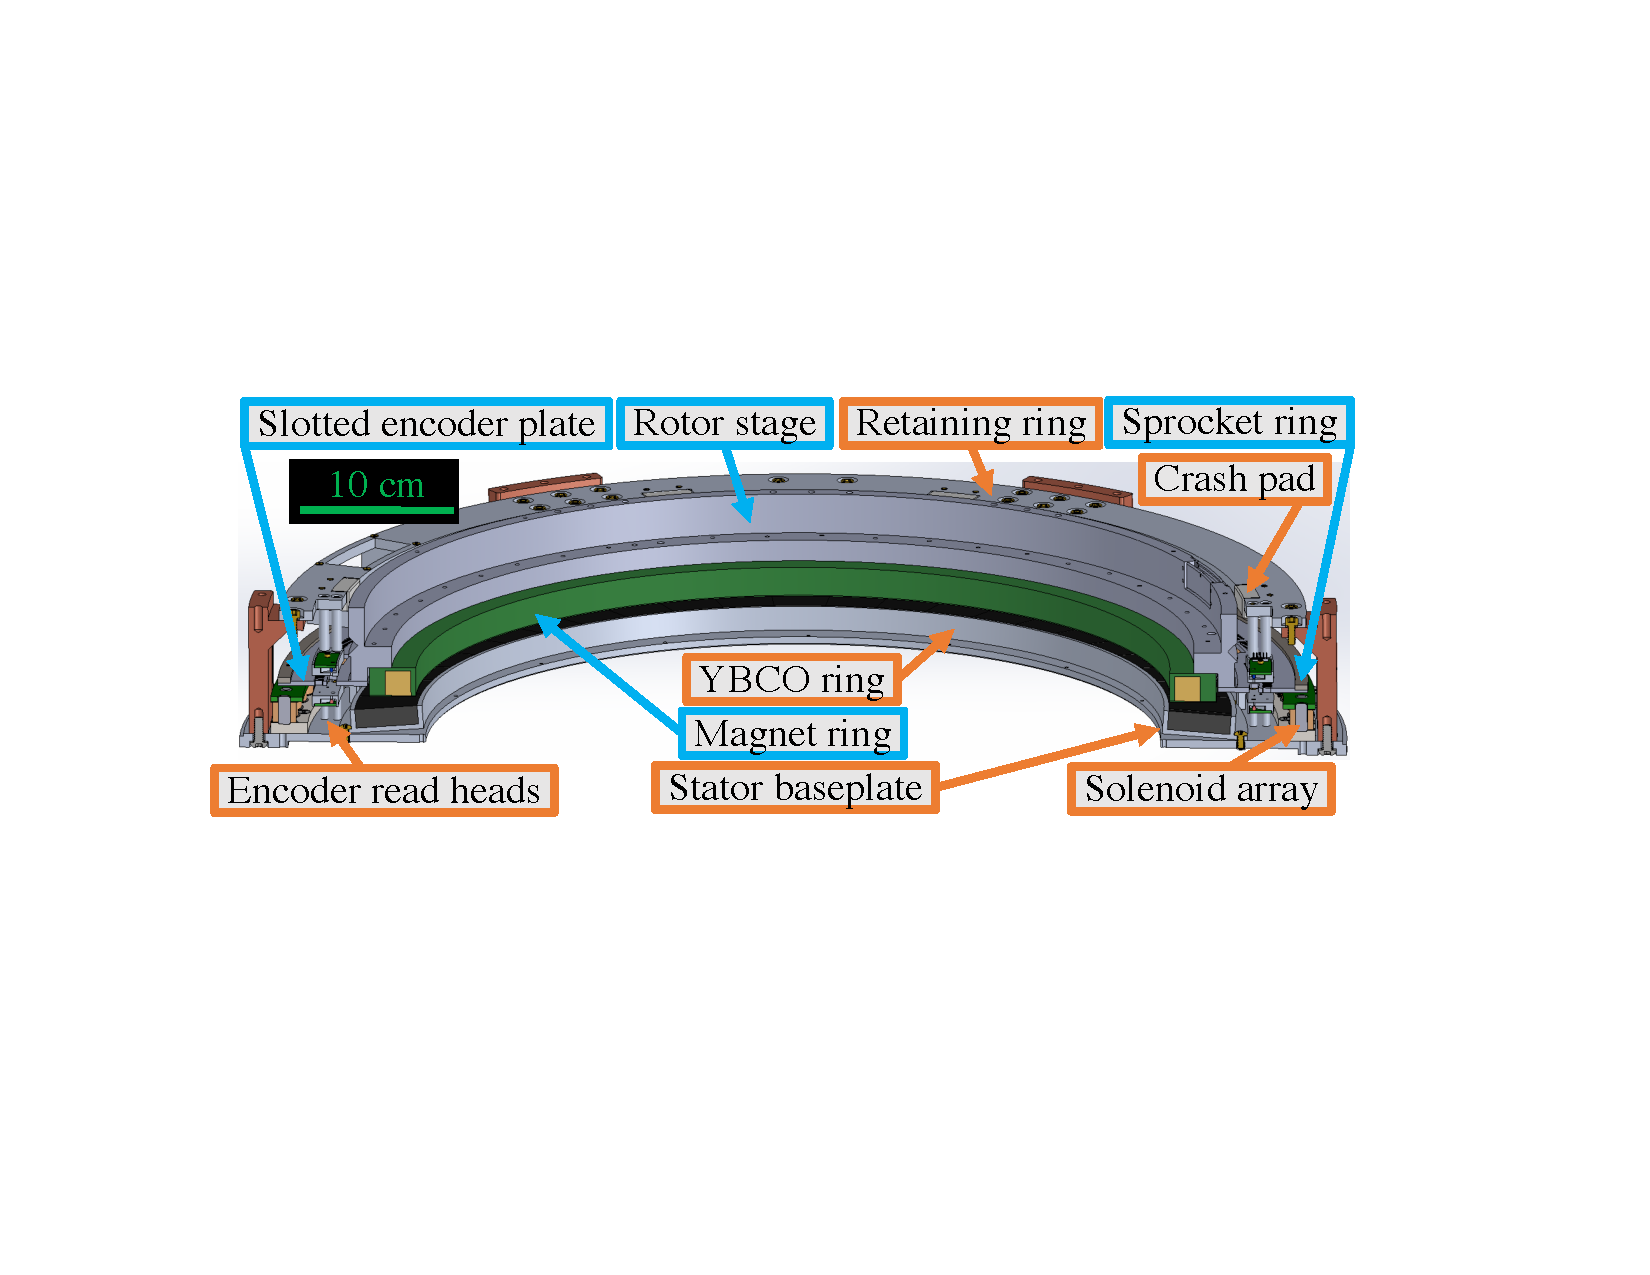
\includegraphics[width=0.75\linewidth, trim={3.5cm, 7.5cm, 4.5cm, 6.5cm}, clip]{CHWPDesign/Figures/CHWP_CAD_standalone_crossSection.pdf}}
    \hfill
    \subfloat[\label{fig:chwp_tabletop:b}]{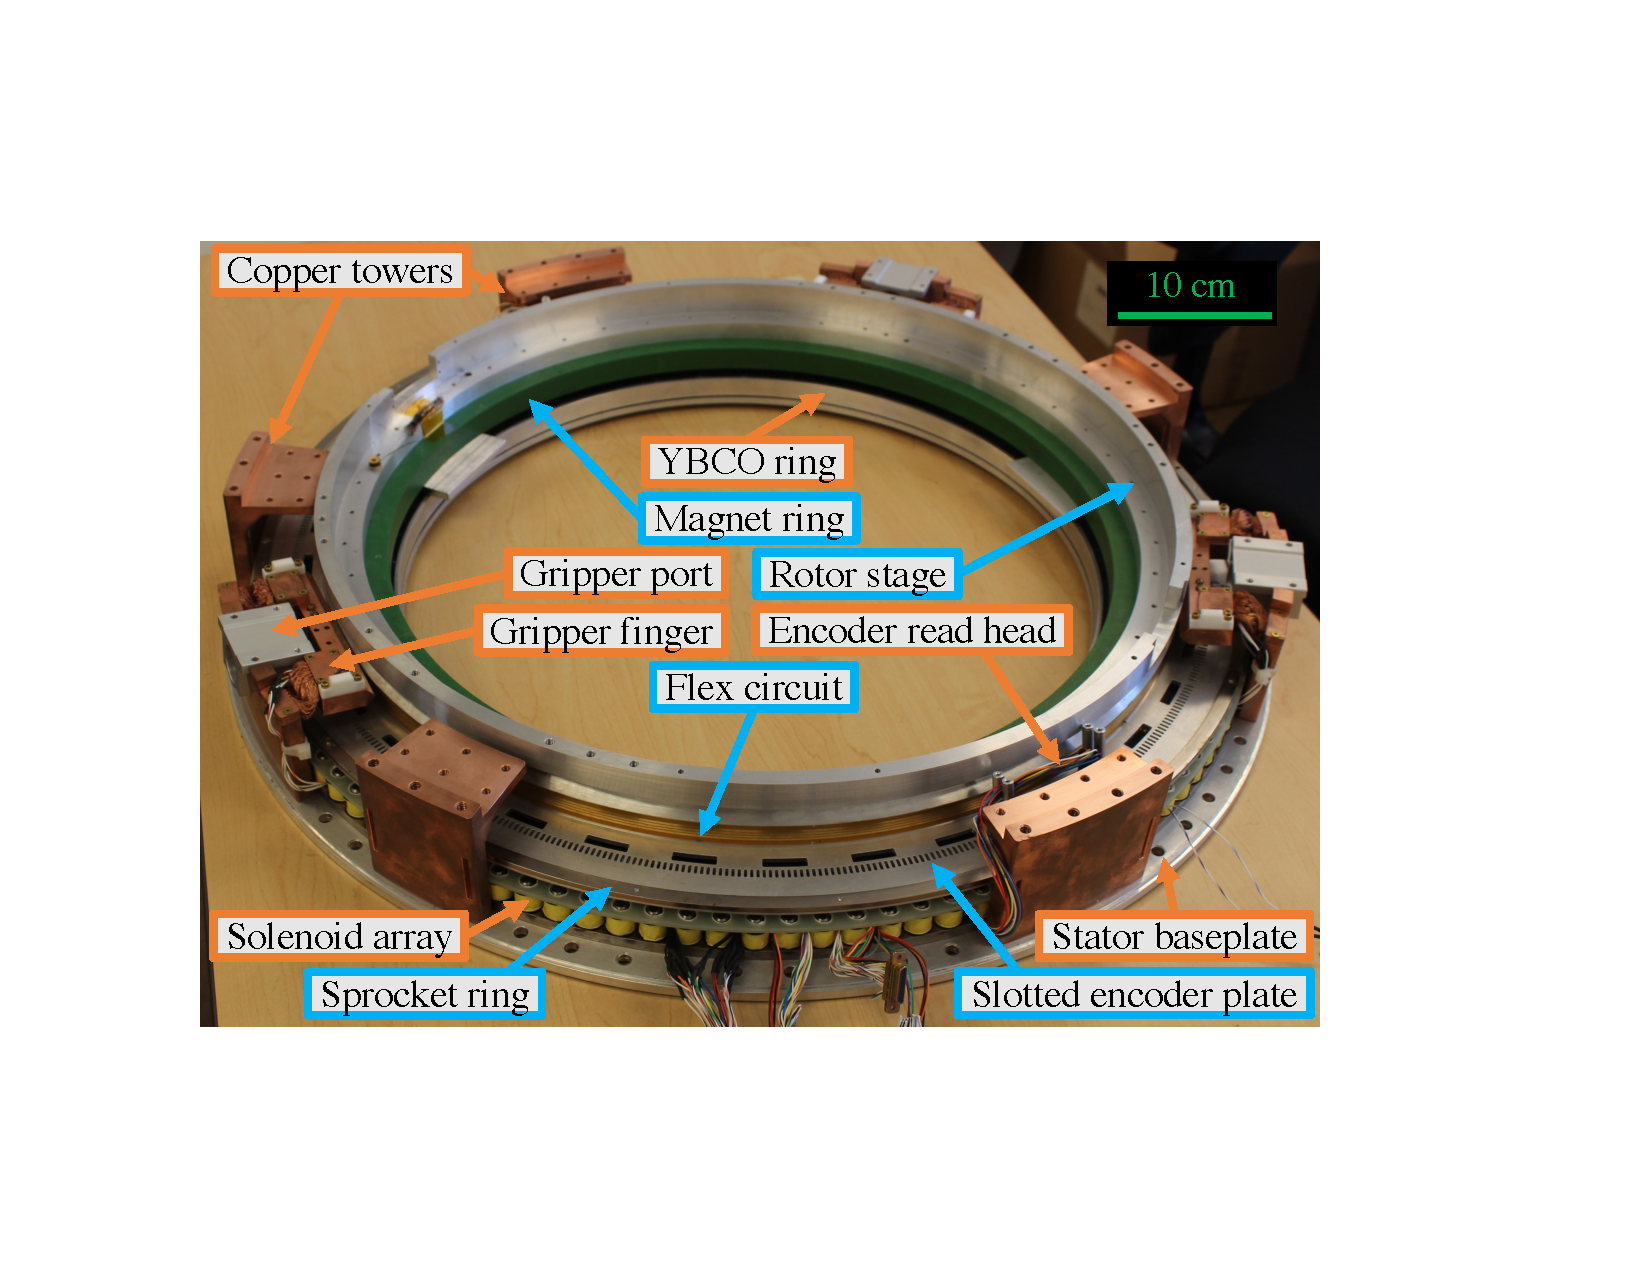
\includegraphics[width=0.75\linewidth, trim={3.5cm, 4.0cm, 5.5cm, 3.5cm}, clip]{CHWPDesign/Figures/CHWP_standalone_photo.pdf}}
    \caption{The CHWP rotation mechanism without the sapphire stack. Rotating components are labeled with cyan boxes, and non-rotating components are labeled with orange boxes. \textbf{Top panel:} a CAD cross section of the rotation mechanism with the rotor floating 5~mm above the stator. The YBCO ring is buckled due to residual thermal stress between the YBCO tiles and their aluminum fixture. \textbf{Bottom panel:} a photograph of the rotation mechanism with the retaining ring removed and the gripper ports, gripper fingers, and flex circuit added. The magnet and YBCO rings are separated by three 4~mm shims. All internal wiring, including that of the solenoids, photodiodes, LEDs, and thermometers, exit the assembly via four 25-pin Micro-D connectors at the bottom of the photo.}
    \label{fig:chwp_tabletop}
\end{figure}

%%%%%%%%%%%%%%%%%%%%%%%%%%%%%%%%
%%%%%%%%%%%%%%%%%%%%%%%%%%%%%%%%

\subsection{Optical design}
\label{sec:optical_design}

As shown in Fig.~\ref{fig:pb2b_chwp_in_ot_cad:b}, the CHWP sapphire stack consists of three $\approx$~505~mm diameter, 3.8~mm-thick sapphire windows\footnote{Guizhou Haotian Optoelectronics Technologies: http://www.ghtot.com/} with a $\approx$~0.7~mm thick dual-layer AR coating on each of its outermost surfaces. The stack is held in an aluminum cradle, which uses tubular springs\footnote{Spira Manufacturing Corporation: https://www.spira-emi.com/} to absorb differential thermal contraction and keep the sapphire from shifting during cooldown and rotation. The cradle has a 490~mm clear aperture diameter, is 20~mm thick, and weighs $\approx$~10~kg including the sapphire stack.

The CHWP's clear aperture is defined by a stationary 440~mm diameter tube lined with HR-10 absorber.\footnote{Eccosorb: https://www.laird.com/rfmicrowave-absorbers-dielectrics} The aperture tube is 60~mm tall and forms a 5~mm gap with the back face of the sapphire stack, ``hiding'' non-optical components from the telescope's beam and restricting the propagation of any CHWP-induced stray light. The CHWP's aperture diameter is limited by bearing manufacturing constraints (see Sec.~\ref{sec:bearing}) yet meets the 430~mm requirement while providing 5~mm of radial alignment tolerance. 

%%%%%%%%%%%%%%%%%%%%%%%%%%%%%%%%
%%%%%%%%%%%%%%%%%%%%%%%%%%%%%%%%

\subsection{Bearing}
\label{sec:bearing}

The CHWP bearing needs to be low-friction, have a large bore diameter, and be mechanically robust at low temperatures. Cryogenic ball bearings with a $\sim$~500~mm bore are not commercially available and are challenging to develop due to thermal contraction, vibration, and durability issues. Therefore, the PB-2b CHWP employs a superconducting magnetic bearing (SMB), as shown in Fig.~\ref{fig:chwp_tabletop}. The SMB operates by flux pinning in an azimuthally symmetric geometry. When suspending a uniformly magnetized ring (the rotor) above a type-II superconducting ring (the stator) and subsequently cooling the superconductor below its transition temperature, the rotor's permanent magnetic field becomes trapped in the stator's superconducting bulk, constraining the rotor in the axial and radial directions while allowing it to rotate in azimuth. SMBs are implemented in other CHWP systems for CMB observation \cite{matsumura_cosmic_2006,klein_cryogenic_2011,sakurai_estimation_2017,Sakurai2018a,Sakurai2020} and their cryogenic robustness is well demonstrated.

The PB-2b SMB is manufactured by Adelwitz Technologiezentrum GmbH.\footnote{ATZ: http://www.atz-gmbh.com/} The magnet ring consists of 16 $22.5^{\circ}$, 97~mm~$\times$~16~mm annular segments of Neodymium (NdFeB), glued contiguously into an encapsulating G10 fixture to form a highly uniform, $\approx$~5,000~G surface field. The superconducting ring consists of 46 $7.8^{\circ}$, 35~mm~$\times$~13~mm annular segments of yttrium barium copper oxide (YBCO), which has a $T_{\mathrm{c}} \approx 90$~K, glued into an encapsulating aluminum fixture to form a contiguous type-II superconductor. Both the rotor and stator have a 470~mm inner diameter, which is large enough to fit around the aperture tube with a 5~mm radial clearance (see Figure~\ref{fig:pb2b_chwp_in_ot_cad:b}).

The SMB's effectiveness relies on a small separation between the permanent magnet and YBCO. SMB stiffness is a steep function of rotor-stator separation \cite{hull_effect_2000}, and therefore controlling the rotor's axial position near the YBCO's transition temperature is critical to controlling the SMB's spring constant. The nominal rotor-stator separation in the PB-2b CHWP system is 5~mm, for which we measure a bearing spring constant of $\approx$~300~N/mm. In addition, SMB friction must be small enough both to achieve the required rotation speed and to mitigate heat dissipation. Eddy losses are induced by eddy currents in nearby metal and scale as $\Delta B^{2}$ \cite{bean_magnetization_1964}, where $\Delta B$ is the rotor's peak-to-peak magnetic field variation. Hysteresis losses arise due to paramagnetic hysteresis in the YBCO and scale as $\Delta B^{3}$ \cite{zeisberger_losses_1998}. Therefore, the uniformity of the magnet ring is critical to minimizing dissipation during continuous rotation. A measurement of rotor friction is presented in Section~\ref{sec:pb2a_chwp_evaluation_thermal_impact}.

%%%%%%%%%%%%%%%%%%%%%%%%%%%%%%%%
%%%%%%%%%%%%%%%%%%%%%%%%%%%%%%%%

\subsection{Gripper}
\label{sec:gripper_design}

Magnetic levitation is a cryogenic phenomenon, and the SMB only engages below the YBCO's $\approx$~90~K superconducting transition temperature. Above this temperature, the YBCO does not flux pin, and the rotor is effectively decoupled from the stator. Therefore, the CHWP employs a ``gripper'' to support the rotor during cooldown and keep it aligned until levitation initiates. The gripper consists of three subassemblies azimuthally distributed about the rotor (see Figure~\ref{fig:chwp_in_pb2b}): one along $-y$, and the others $\pm$~40~deg\footnote{The opening angle of the top two subassemblies is less than $120^{\circ}$ to avoid mechanical interference with the optics tube's PTR attachment.} about $+y$. Each subassembly has a linearly actuating vacuum feedthrough at 300~K, a flexible, thermally isolating ``arm'' between 300 and 50~K, and a 50~K ``finger'' that engages the rotor stage.  When the gripper fingers are extended, the rotor is gripped, and when they are retracted, the rotor is released.

\begin{figure}[!t]
    \centering
    \subfloat[\label{fig:gripper_assy}]{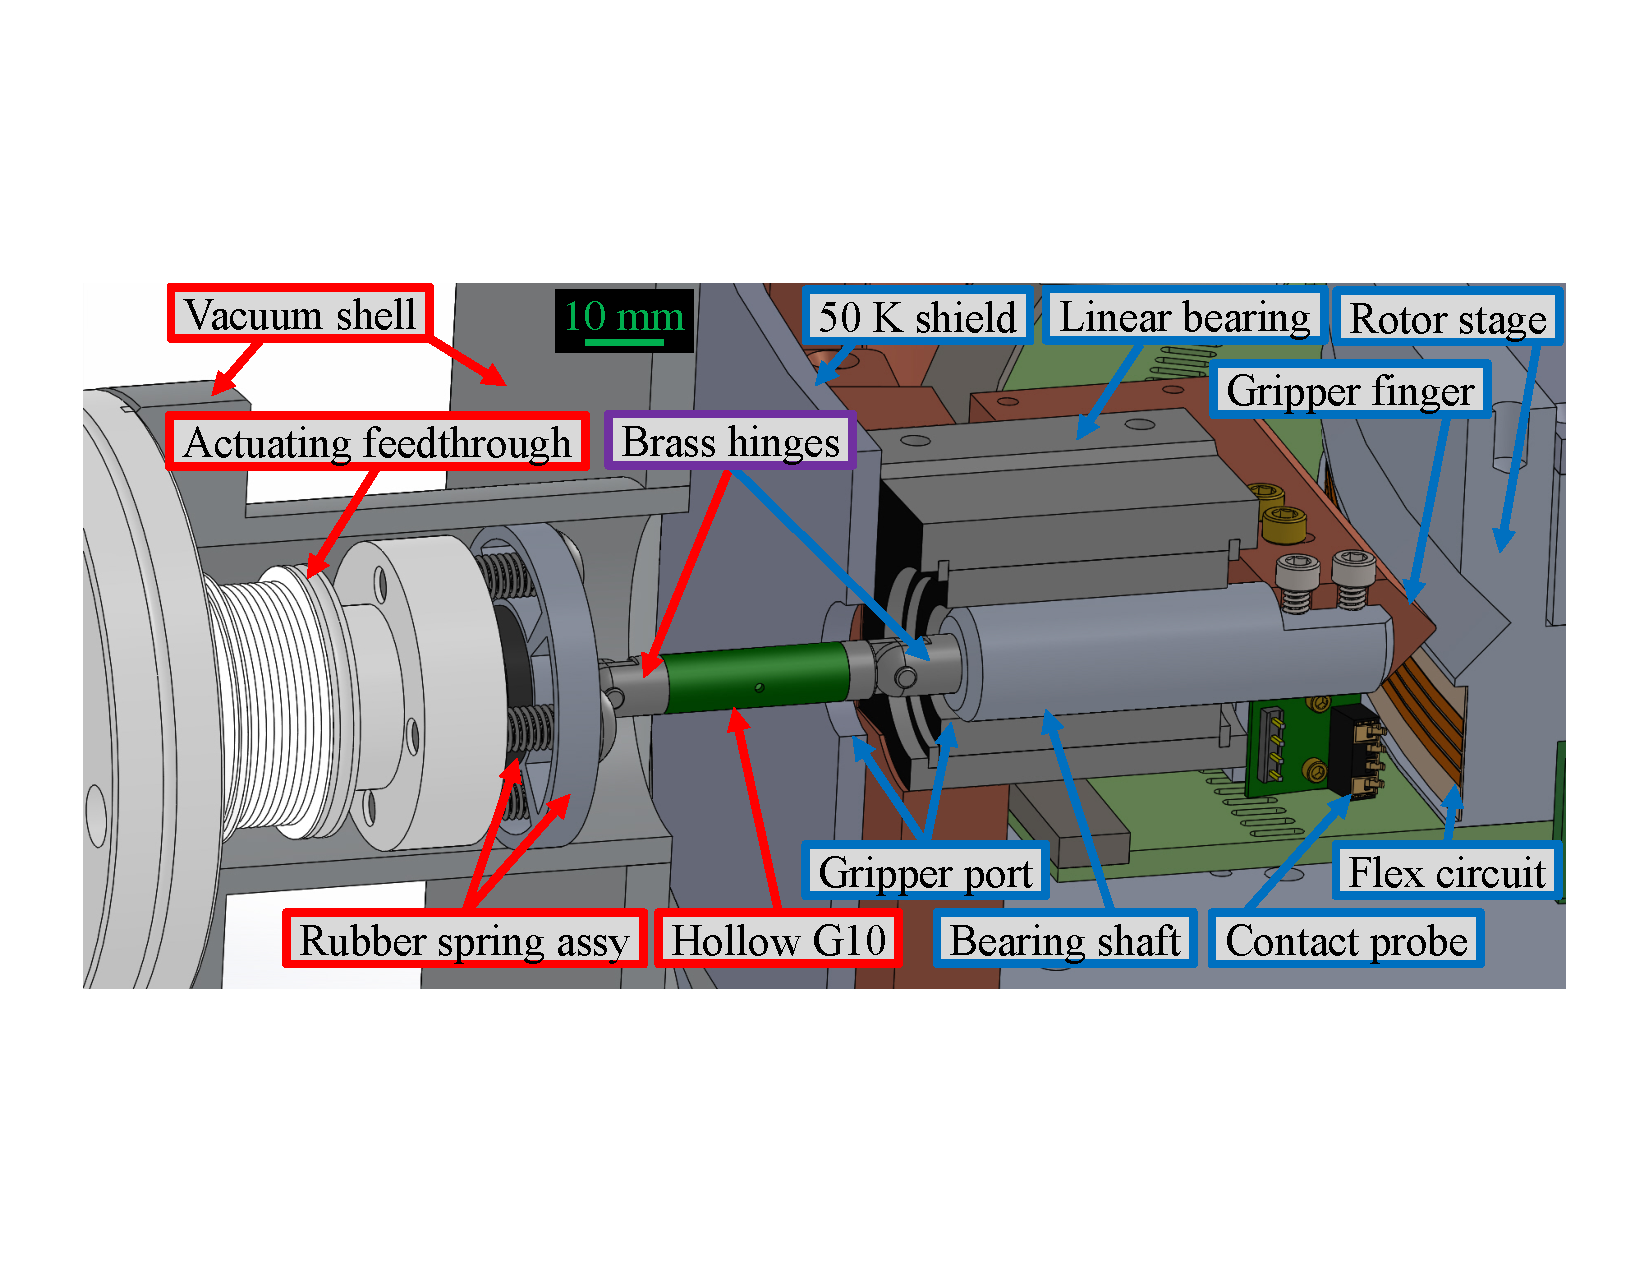
\includegraphics[width=0.7\linewidth, trim=2cm 4cm 1.4cm 4.2cm, clip]{CHWPDesign/Figures/gripper_CAD_crossSection.pdf}}
    \hfill
    \subfloat[\label{fig:gripper_assy:b}]{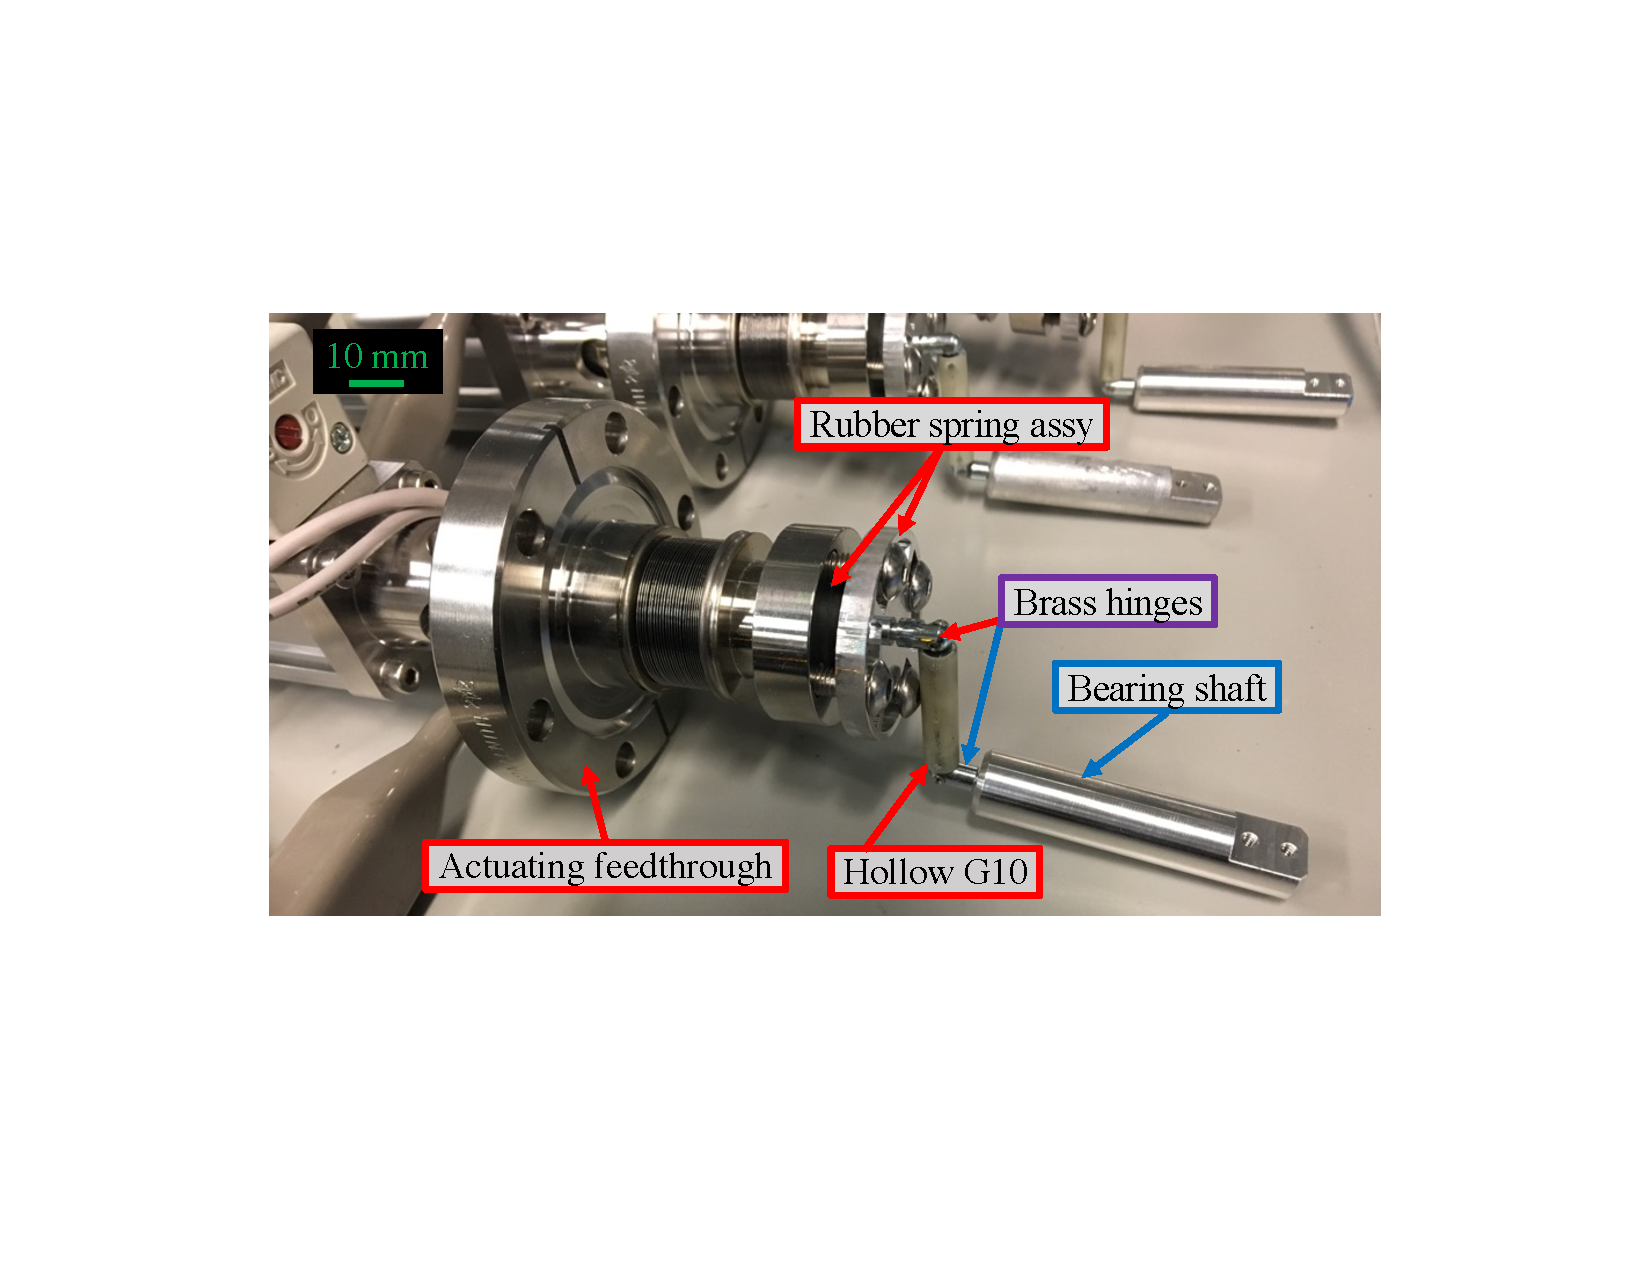
\includegraphics[width=0.5\linewidth, trim=4.5cm 4.3cm 4.5cm 5cm, clip]{CHWPDesign/Figures/gripperMotor_photo.pdf}}
    \subfloat[\label{fig:gripper_assy:b}]{\includegraphics[width=0.5\linewidth, trim=5cm 5cm 5.8cm 3.5cm, clip]{CHWPDesign/Figures/gripperPort_photo.pdf}}
    \caption{A detailed view of a single gripper subassembly with the retaining ring removed for visual clarity. Red boxes mark warm components, and blue boxes mark cold components. \textbf{Top panel:} a CAD cross section of a gripper subassembly with the rotor un-gripped and floating.  \textbf{Middle panel:} a photograph of a feedthrough actuator attached to a gripper arm. \textbf{Bottom panel:} a photograph of the linear bearing and the copper gripper finger without the gripper arm.}
    \label{fig:gripper_assy}
\end{figure}

Figure~\ref{fig:gripper_assy} shows a CAD rendering and photographs of a single gripper subassembly. The feedthrough\footnote{Huntington Mechanical Laboratories: https://huntvac.com/} consists of a linear actuator\footnote{SMC Corporation: https://www.smcusa.com/} with a vacuum-compatible bellows assembly that mounts to a ConFlat port on the vacuum shell. The feedthrough bolts to a rubber spring assembly, which adds compliance both along and about the radial direction. This spring assembly in turn connects to the gripper arm, which is composed of a hinged thermal isolator joined to a 6~mm diameter, 50~mm long aluminum bearing shaft. The thermal isolator comprises two brass hinges epoxied to either end of a 24~mm long, 0.8~mm-thick-walled hollow G10 tube. The hinges accommodate differential thermal contraction along the receiver cryostat's axial direction and relax alignment tolerances between the 300~K and 50~K stages.

The bearing shaft enters the 50~K assembly through a gripper port, which includes a 10~mm diameter hole in the 50~K shield and a Frelon-lined linear bearing within which the bearing shaft slides. Because this port introduces a potential 300~K light leak, the outer surface of the linear bearing and the inner surface of the 50~K shield are blackened with carbon-loaded Stycast \cite{persky_review_1999} to limit the propagation of any stray light. The innermost end of the bearing shaft bolts to the gripper finger, which is a 6~mm deep, $90^{\circ}$-angled, oxygen-free high-thermal-conductivity (OFHC) copper wedge, attached to the CHWP stator via two flexible OFHC copper-braid heat straps. When the rotor is gripped, the finger fits into an identically shaped, azimuthally symmetric groove on the rotor stage, heat sinking the rotor while constraining its axial position.

The gripper finger also contains a spring-loaded probe that contacts an azimuthally symmetric flex circuit when the rotor is gripped, permitting four-point readout of a silicon diode thermometer\footnote{Lakeshore DT-670: https://www.lakeshore.com} on the sapphire stack's cradle. The probe is a beryllium copper, four-point battery contact, and the Kapton-based flex circuit\footnote{Q-Flex: https://www.qflexinc.com/} has four 2~mm-wide, 2.5~mm-pitch, gold-plated copper traces soldered to the thermometer's leads.

The complete gripper assembly is composed of three subassemblies that actuate simultaneously to grip and release the rotor. The motors are driven by a parallel-output controller,\footnote{SMC JXC-831: https://www.smcpneumatics.com/JXC831.html} which is commanded using a programmable logic controller (PLC). The typical cooldown configuration for the PB-2b receiver is approximately horizontal (see Figure~\ref{fig:chwp_in_pb2b}), with the bottom gripper finger supporting the rotor's 17~kg mass during cooldown. Therefore, we employ a 450~N-max motor for the bottom subassembly and 200~N-max motors for the top two.\footnote{SMC LEY-32 and LEY-16: https://www.smcusa.com/}

The gripper is designed for reliability. Each gripper finger attaches to its bearing shaft with two titanium bolts to avoid fastener fatigue and has two PTFE stabilizers that slide along the bottom face of the retaining ring (see Figure~\ref{fig:chwp_tabletop}) to constrain rotation about the gripper-port axis. The G10 tubes and hinges are joined with a step to avoid compression failures, and the hinges are screened to withstand more than four times the rotor's weight. In addition, the rotor's center of mass lies in the plane of its triangular groove, and the bottom finger's copper wedge is slightly V-shaped, forming a $176^{\circ}$ angle about the radial direction. These two features allow the rotor to be constrained by the bottom subassembly alone when the receiver is horizontal, hence providing insurance against possible gripper failure modes such as motor control issues and imperfect subassembly synchronization.

%%%%%%%%%%%%%%%%%%%%%%%%%%%%%%%%
%%%%%%%%%%%%%%%%%%%%%%%%%%%%%%%%
%%%%%%%%%%%%%%%%%%%%%%%%%%%%%%%%

\section{Motor}
\label{sec:motor_design} 

The CHWP motor needs to drive stable 2~Hz rotation while being low-dissipation, low-magnetic-interference, and mechanically robust at cryogenic temperatures. While a belt drive with an external motor has been successfully operated during weeks of CMB observation \cite{klein_cryogenic_2011,the_ebex_collaboration_ebex_2018}, the PB-2b CHWP must run for years, motivating a drive system free of mechanical fatigue. Therefore, we utilize a brushless, three-phase, synchronous electromagnetic motor driven by custom electronics. We discuss the motor's cryogenic assembly, driver, and efficiency in the following subsections.

%%%%%%%%%%%%%%%%%%%%%%%%%%%%%%%%
%%%%%%%%%%%%%%%%%%%%%%%%%%%%%%%%

\subsection{Motor cryogenic assembly}
\label{sec:motor_mech} 

The motor's cryogenic assembly is shown in Figure~\ref{fig:motor_mech_assy}. Its active component consists of 114 solenoids\footnote{APW Company: https://apwelectromagnets.com/fc-6035.html} with low-carbon-steel magnetic cores glued with equal spacing onto a 650~mm diameter low-carbon-steel ring on the stator. Each coil has an 8.6~mH inductance and a $\approx$ 3~$\Omega$ resistance at 50~K, and the motor's three phases are driven across three regularly interspersed groups of 38 coils. In order to reduce the motor's equivalent resistance and hence reduce the voltage needed to operate it, the solenoid array is further divided into four sections---two with 30 total coils, two with 27 total coils---that are driven in parallel. The motor's passive component consists of 76 1.5~mm diameter $\times$ 1.5~mm tall NdFeB magnet sprockets, which have a 6,700~G surface field and are glued with equal spacing and alternating polarity onto a 650~mm diameter low-carbon-steel sprocket ring on the rotor.

\begin{figure}[!t]
    \centering
    \subfloat[\label{fig:motor_mech_assy:a}]{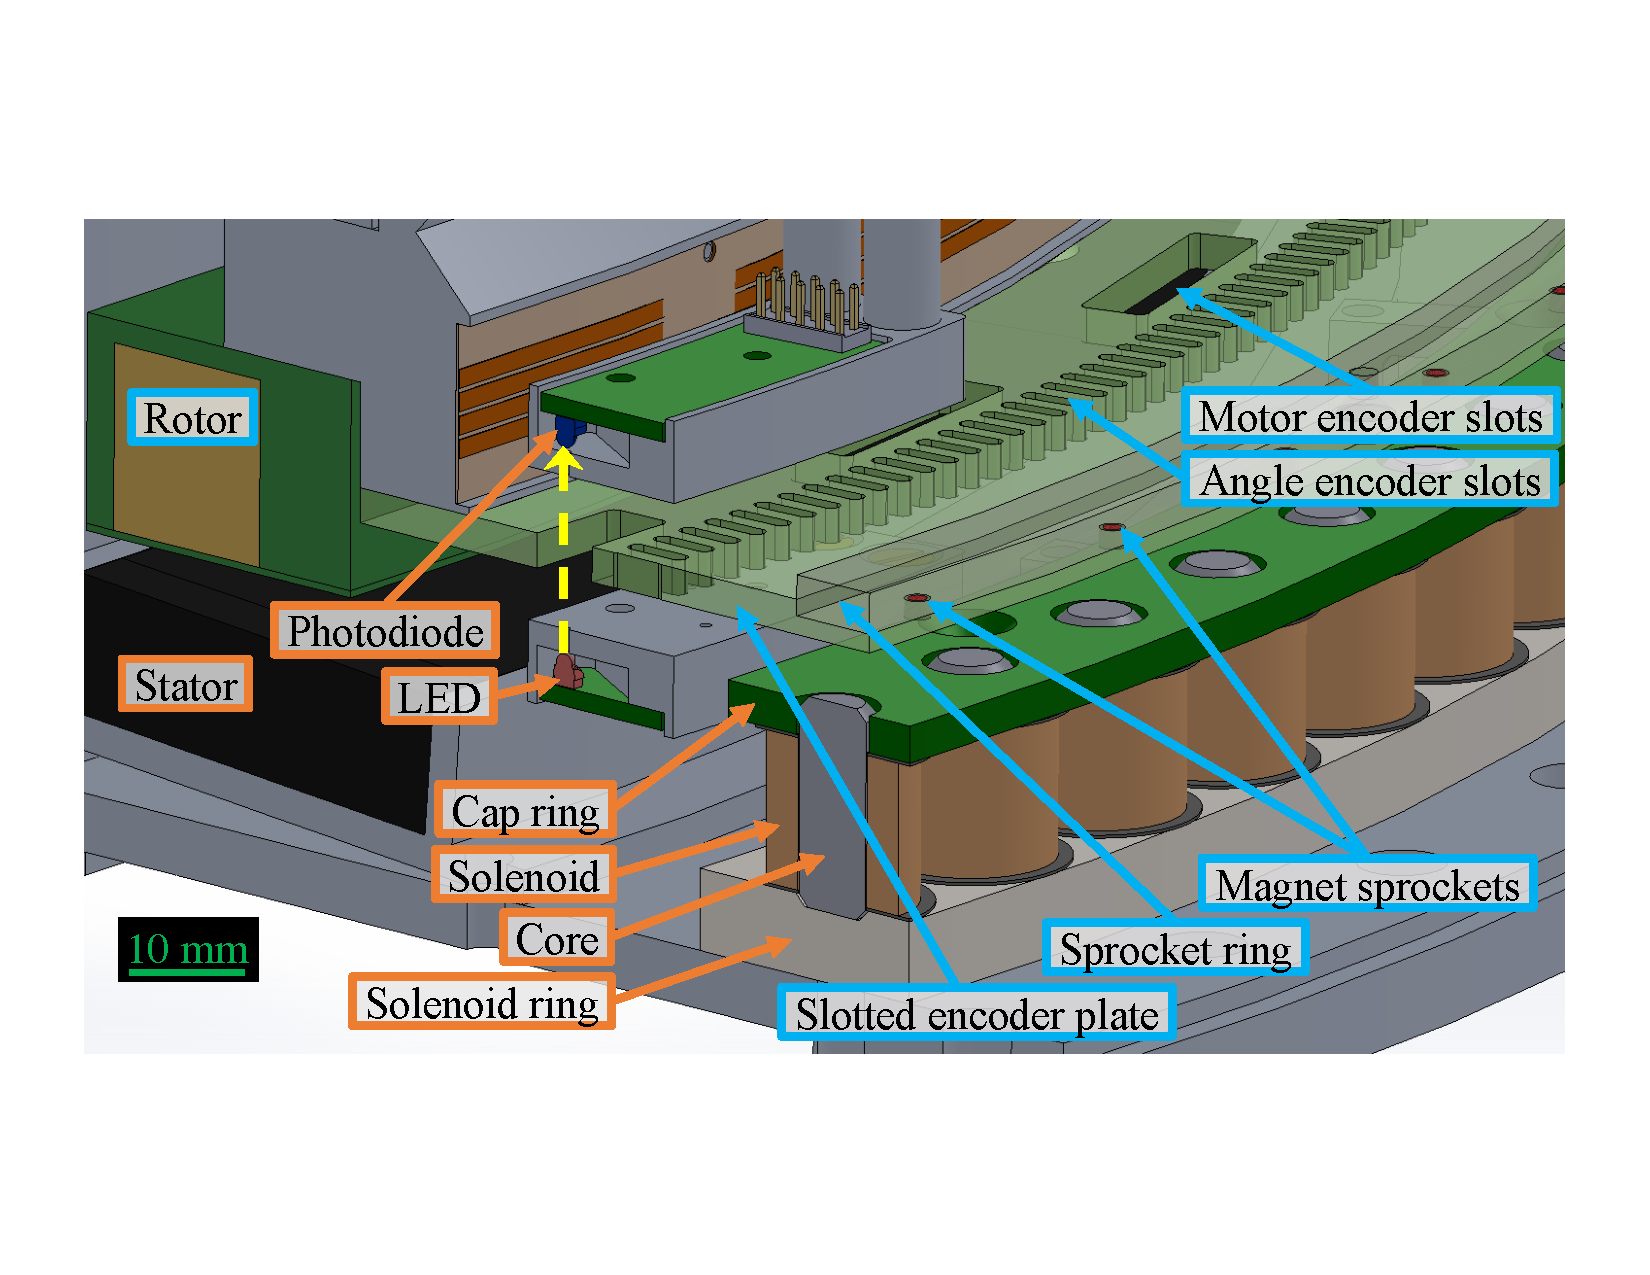
\includegraphics[width=0.5\linewidth, trim=1cm 3cm 1cm 3cm, clip]{CHWPDesign/Figures/motorEncoder_CAD_crossSection.pdf}}
    \subfloat[\label{fig:motor_mech_assy:b}]{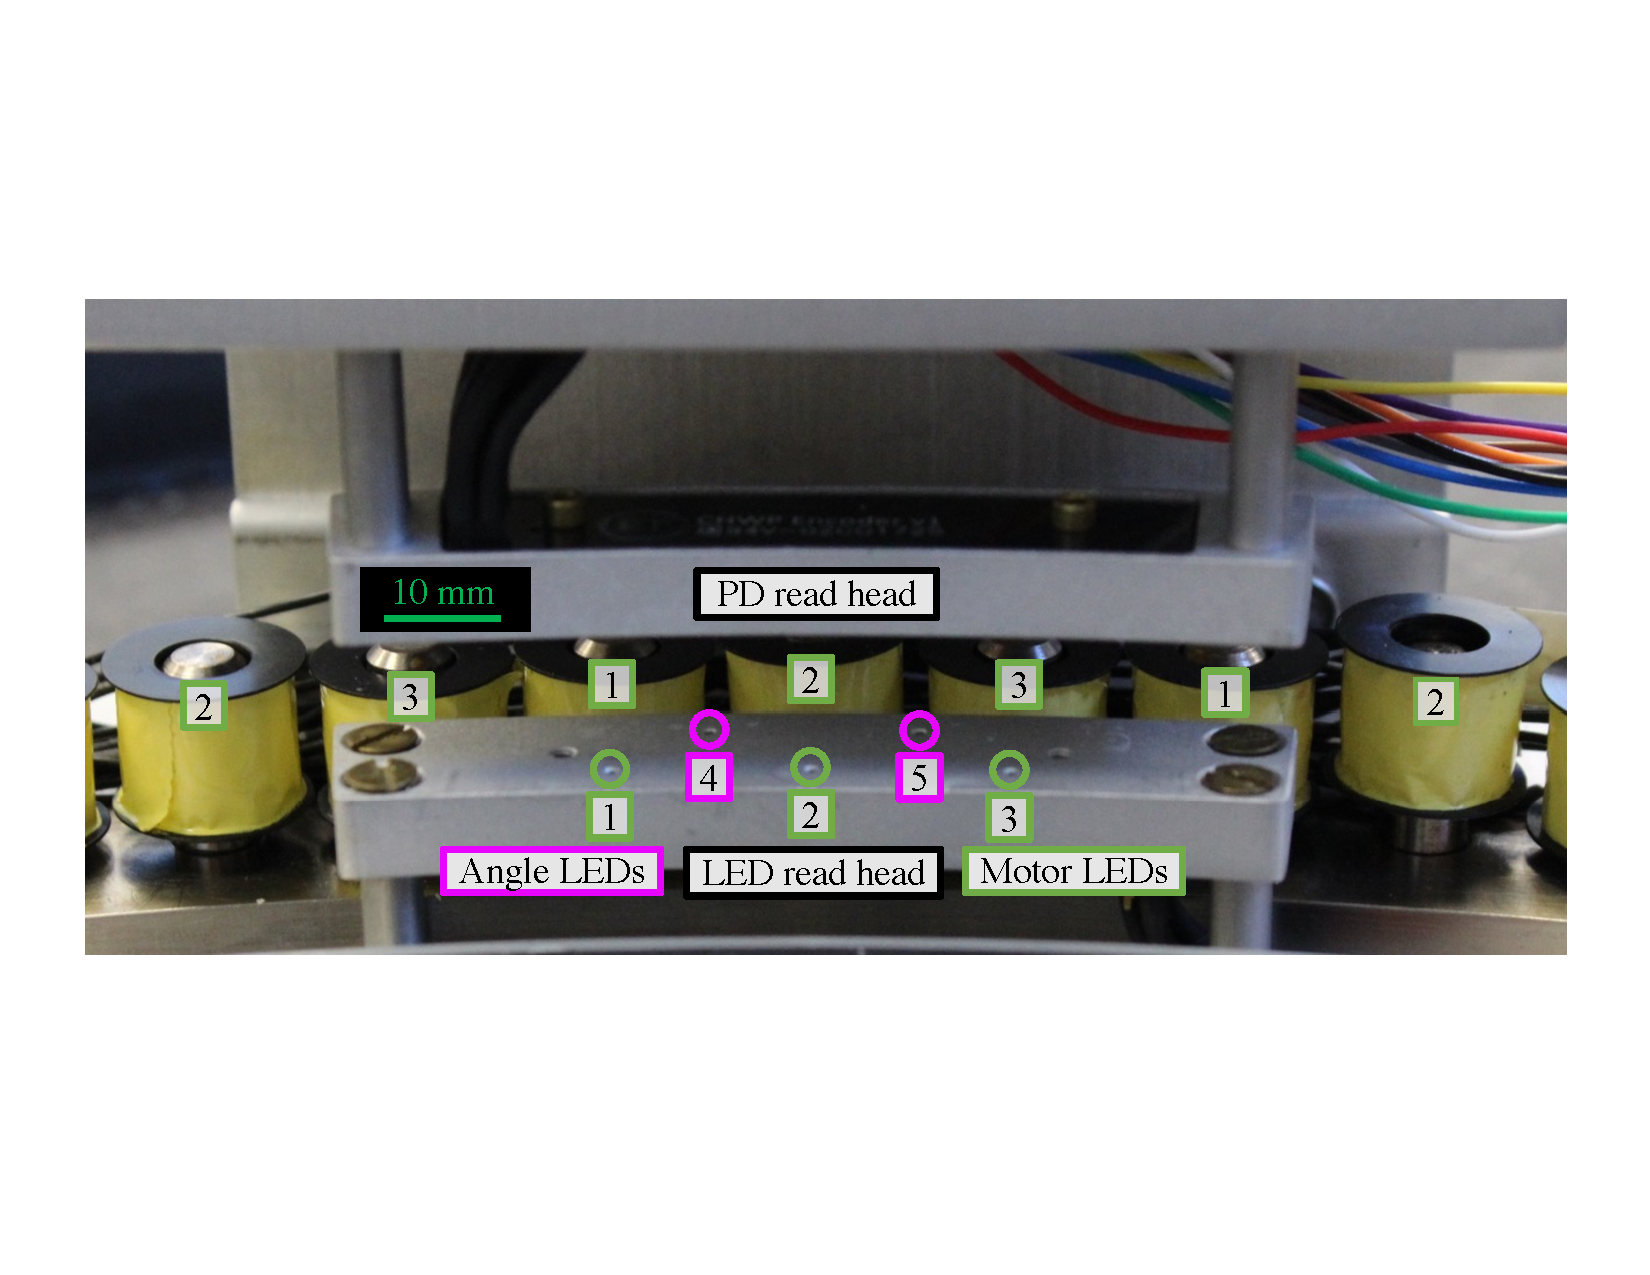
\includegraphics[width=0.5\linewidth, trim=4.5cm 3.8cm 4.5cm 7.5cm, clip]{CHWPDesign/Figures/encoderReadhead_photo.pdf}}
    \caption{\textbf{Top panel:} a zoomed CAD cross section of the CHWP motor. Rotating components are labeled with cyan boxes, and stationary components are labeled with orange boxes. The slotted encoder plate and sprocket ring are semi-transparent for visual clarity. \textbf{Bottom panel:} a photograph of the encoder read heads and nearby solenoids with the slotted encoder plate removed. The collimator holes for the motor LEDs are circled in green and labeled by phase, while those of the angle LEDs are circled in magenta. The solenoids are also labeled by phase and are radially aligned with their corresponding motor LED-PD pairs.}
    \label{fig:motor_mech_assy}
\end{figure}

The solenoids are energized in three $120^{\circ}$-separated phases with an alternating drive voltage $\pm \; \mathrm{V_{D}}$, creating an oscillating magnetic field that couples to the rotor's magnet sprockets, driving rotation. The sprockets, solenoids, and cores are carefully chosen to avoid cogging while providing enough torque to attain the required rotational velocity. At 2~Hz rotation, the motor delivers only $\approx$~5~N-mm of torque, making it susceptible to physical touches. Therefore, the CHWP assembly includes a system of wire harnesses to facilitate clean cable management. Additionally, despite the $<$~2~mm rotor-stator alignment requirement presented in Section~\ref{sec:motor_eff}, we provide 5~mm of clearance around the rotor to further limit the possibility of a physical touch impacting rotation.

The coils are driven by custom electronics, described in Section~\ref{sec:driver}, whose sensing component is an optical encoder on the 50~K stage shown in Figure~\ref{fig:motor_mech_assy}. The encoder consists of three 940~nm light-emitting diodes\footnote{Vishay VSMB294008G: \\ https://www.vishay.com/docs/84228/vsmb294008rg.pdf} (LEDs) shining onto three reverse-biased photodiodes\footnote{Vishay TEMD1020: \\ https://www.vishay.com/docs/81564/temd1000.pdf} (PDs) through a slotted encoder plate on the rotor. The LEDs and PDs are soldered to printed wiring boards and are housed in aluminum read heads with 1~mm diameter, 3~mm deep collimation holes. As shown in Figures~\ref{fig:chwp_tabletop} and~\ref{fig:motor_mech_assy}, the LED read head is mounted to four precision-ground aluminum standoffs on the stator baseplate, while the PD read head is similarly mounted to the retaining ring on the opposite side of the slotted encoder plate. Each motor LED-PD pair is azimuthally aligned with the solenoid array, and the read heads are aligned to each other using dowel pins during assembly. The gallium aluminum arsenide LEDs and the silicon PDs are cryogenically screened via dunk tests in liquid nitrogen and have been robust throughout hundreds of hours of testing. Even so, the CHWP has two identical pairs of read heads, as shown on the right- and left-hand sides of Figure~\ref{fig:chwp_tabletop}, to provide insurance against LED or PD failure. The slotted encoder plate has 38 5~mm wide motor slots whose edges are azimuthally aligned to the magnet sprockets. During rotation, the slot pattern chops the PD input, and the motor driver converts this photocurrent waveform into the solenoid bias voltage, as described in the following subsection. Both the slotted encoder plate and cap ring are made of G10 to minimize motor-induced eddy currents on both the stator and rotor.

%%%%%%%%%%%%%%%%%%%%%%%%%%%%%%%%
%%%%%%%%%%%%%%%%%%%%%%%%%%%%%%%%

\subsection{Motor driver}
\label{sec:driver}

The motor drive electronics must be robust, low-noise, and simple to operate. While commercial drivers for synchronous motors are abundant, most involve auxiliary control software, pulse-width-modulated (PWM) waveforms (which can inject high-frequency noise into the receiver), and awkward interfacing to the PB-2b cryogenic assembly. Therefore, we employ a custom driver printed circuit board (PCB) that both meets our requirements and simplifies CHWP operation. The presented PCB is also used to read out the angle encoder signal, which is discussed in Section~\ref{sec:angle_encoder}.

\begin{figure}[!t]
    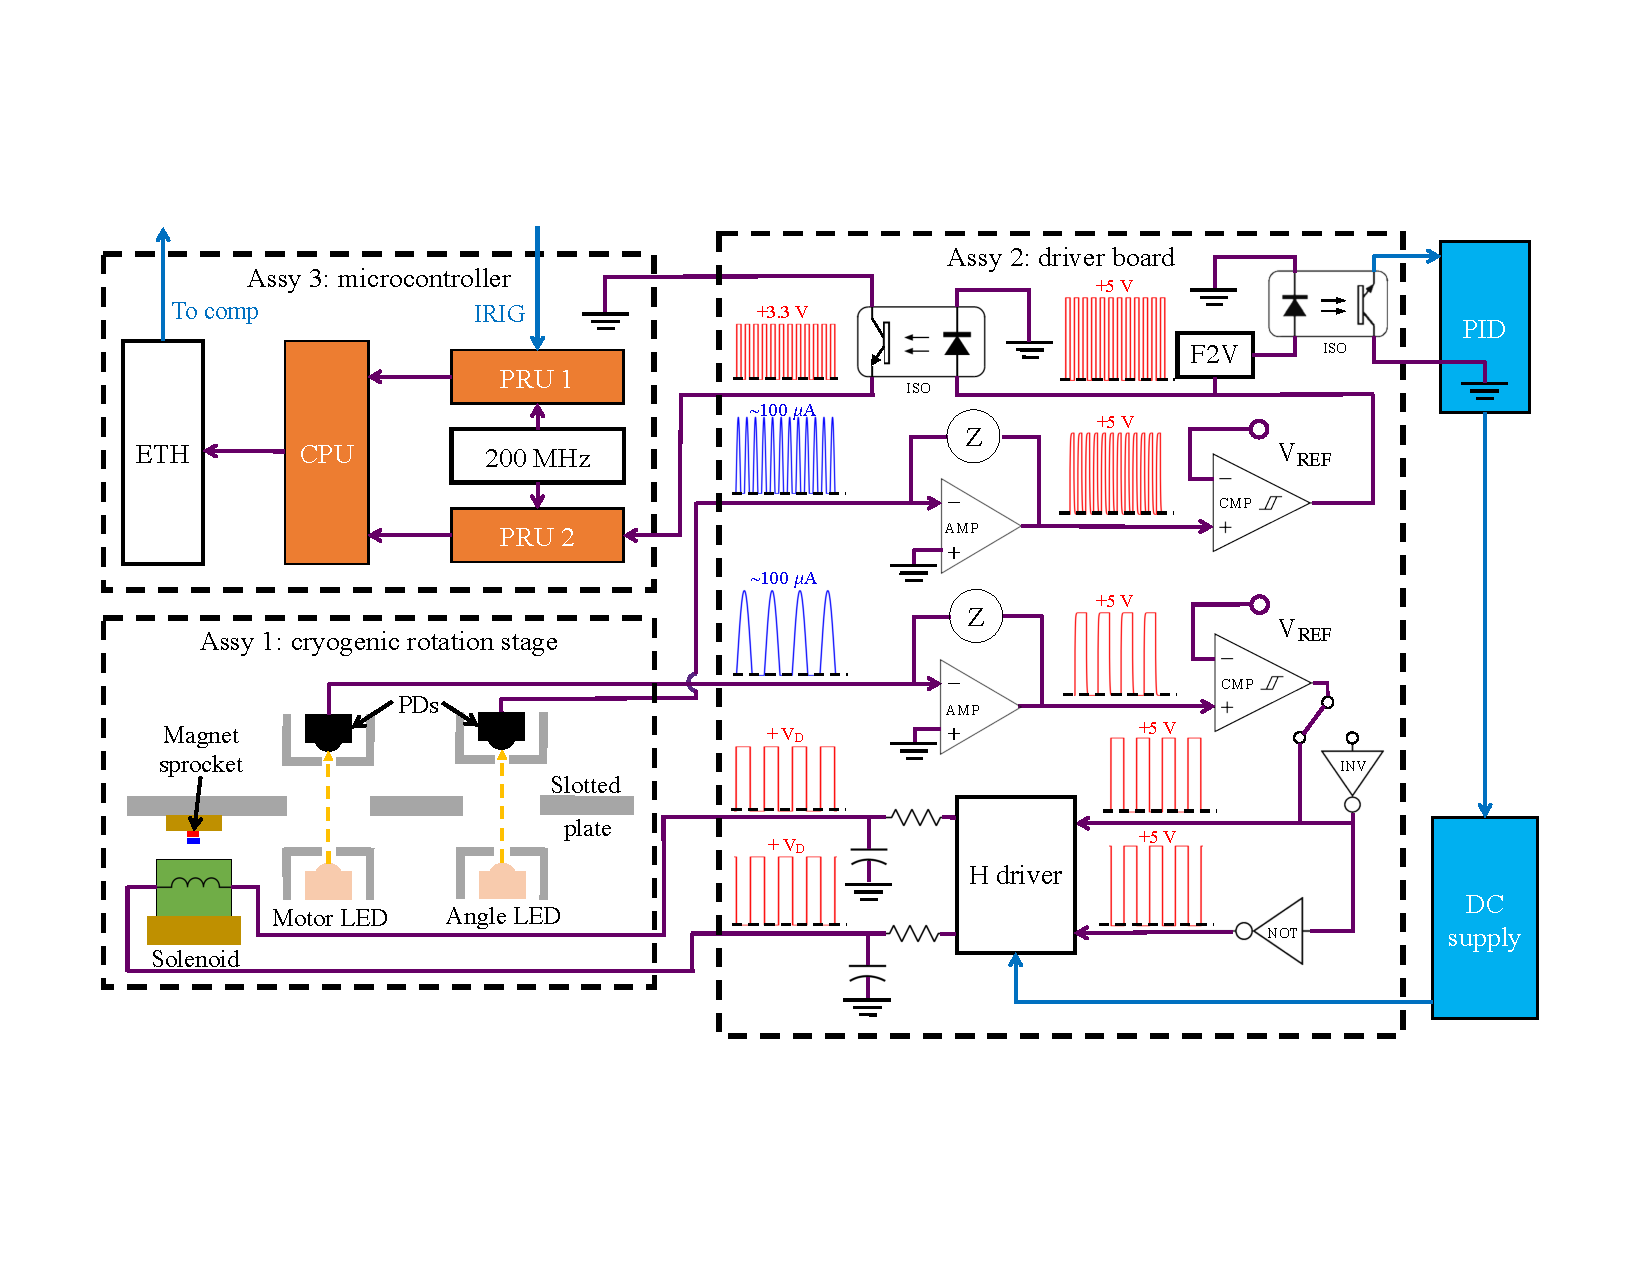
\includegraphics[width=\linewidth, trim=1.5cm 3.8cm 1.5cm 3.5cm, clip]{CHWPDesign/Figures/motorDriver_schematic.pdf}
    \caption{A signal diagram for a single phase of the CHWP motor driver and for a single angle encoder output. On the \textbf{cryogenic rotation stage}, the slotted encoder plate, which has one lane of slots for motor encoding and another for angle encoding, chops the signals of the LED-PD pairs. The \textbf{driver board} converts these photocurrents into voltage signals using transimpedance amplifiers (AMP) with carefully tuned low-pass feedback (Z) and then converts these analog waveforms into 5~V digital signals using comparators (CMP) with potentiometer-tunable reference voltages ($\mathrm{V_{REF}}$). For motor control, both non-inverted and inverted (NOT) signals are passed to an H-bridge driver (H driver), which outputs synchronized, low-pass-filtered, alternating-polarity voltage waveforms $\pm \mathrm{V_{D}}$ to the solenoids. For angle encoder readout, which has a 15$\times$ faster signal than that of the motor, the digital signals are opto-isolated (ISO) and sent to a microcontroller unit for processing. Additionally, the angle encoder digital signal is passed to a frequency-to-voltage converter (F2V) whose opto-isolated output is used by a PID controller to provide feedback to the H-driver voltage and stabilize CHWP rotation. To brake or reverse direction, a switched inverter (INV) applies a global $180^{\circ}$ phase shift to the H-driver input. The \textbf{microcontroller} is a BeagleBone Black, which has two programmable real-time units (PRUs) that share a 200~MHz clock. PRU 1 timestamps and decodes a GPS-synchronized IRIG-B PWM waveform, while PRU 2 timestamps rising and falling edges of the digital angle encoder waveform. These data are written to a shared buffer, which is emptied by the central processing unit (CPU) before being sent to an external computer over Ethernet (ETH).}
    \label{fig:motor_driver_schematic}
\end{figure}

\begin{figure}[!t]
    \centering
    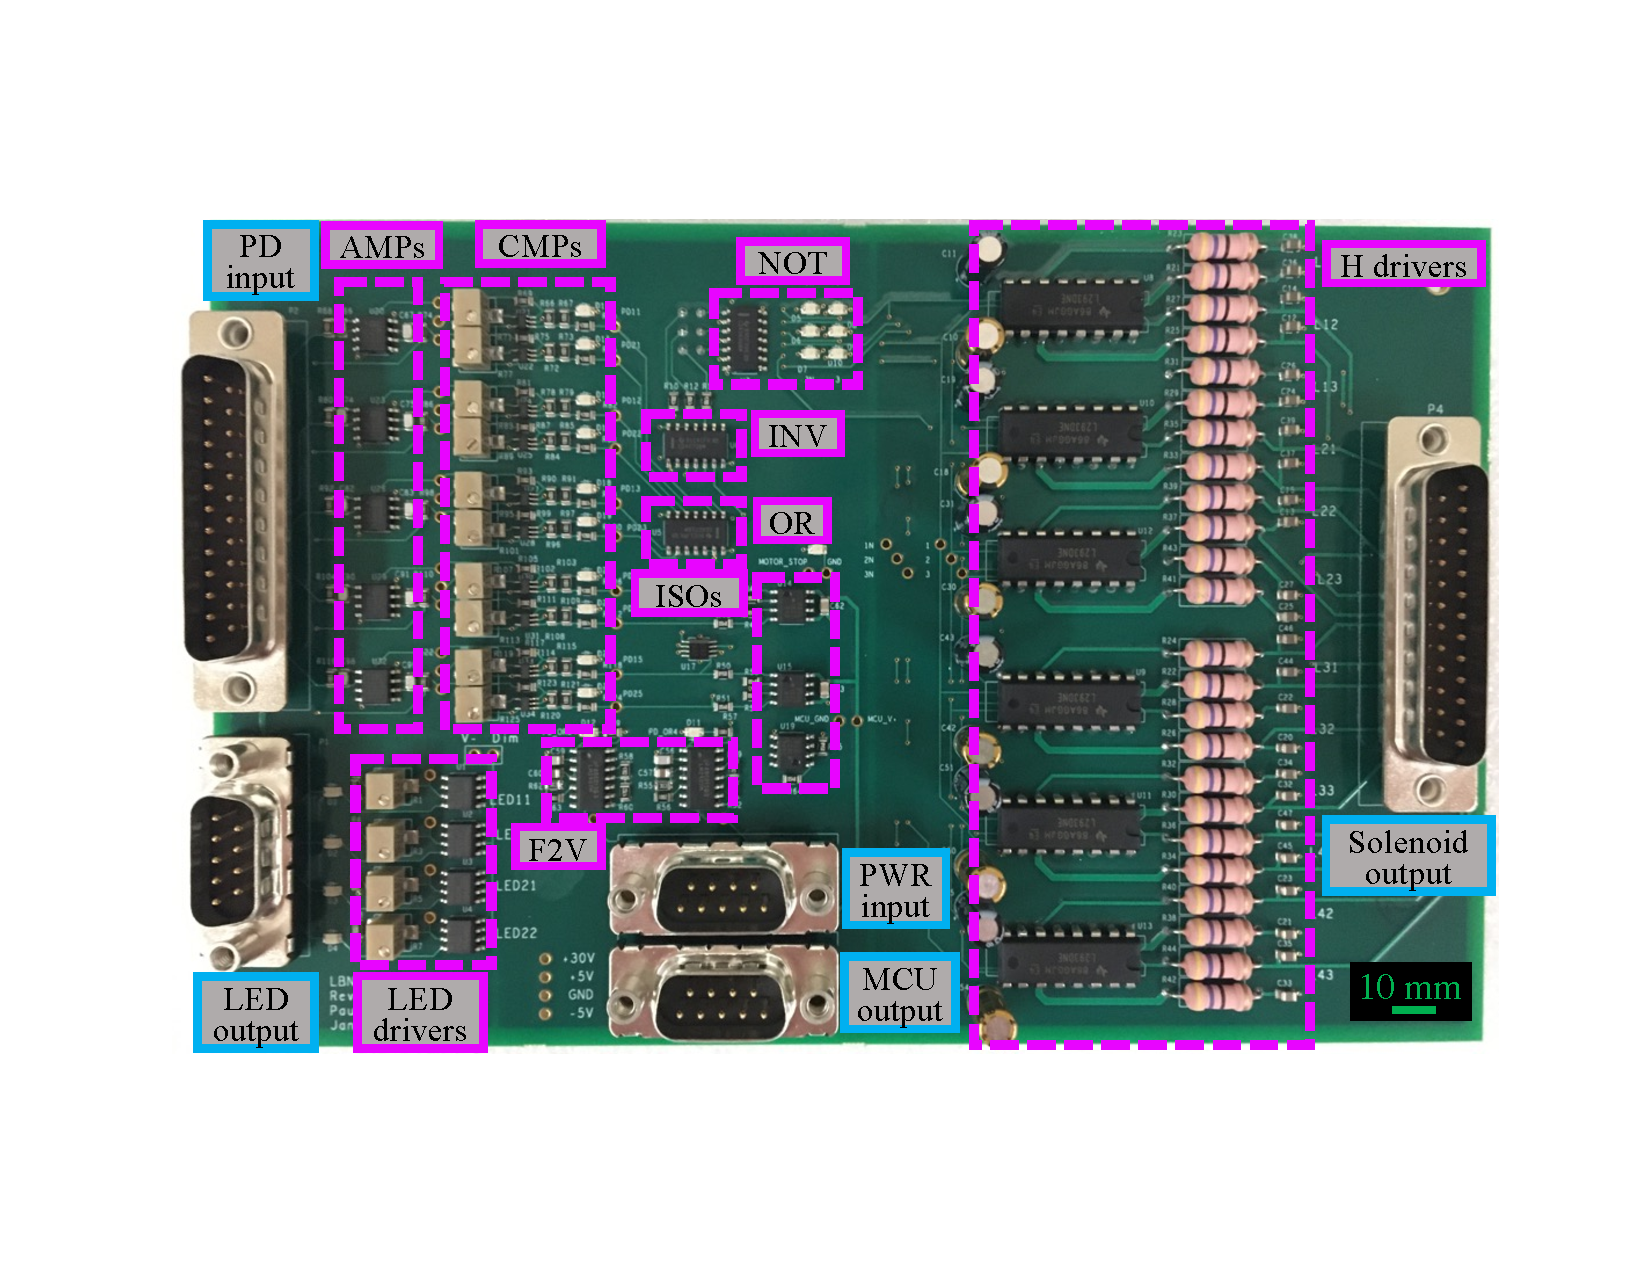
\includegraphics[width=0.7\linewidth, trim=3.0cm 3.5cm 2.5cm 3.6cm, clip]{CHWPDesign/Figures/motorDriver_photo.pdf}
    \caption{A photograph of the driver PCB, the schematic for which a subset is shown in Fig.~\ref{fig:motor_driver_schematic}. The photocurrents from all ten encoder PDs enter the board through the ``PD input'' connector before being converted to analog signals by the transimpedance amplifiers ``AMPs'' and converted to 5~V digital signals by the comparators ``CMPs.'' At this point, the angle encoder signals are opto-isolated (``ISOs'') and sent to the microcontroller via the ``MCU output'' connector. The motor signals from both PD read heads are ``OR-ed'' before being inverted (``INV'') and input to the ``H drivers,'' which in turn power the solenoids via the ``Solenoid output'' connector. The motor and encoder LEDs are current biased by potentiometer-adjustable ``LED drivers'' via the ``LED output'' connector. DC supply voltages come through the ``PWR input'' connector.}
    \label{fig:motor_driver_photo}
\end{figure}

A single PD amplification chain is shown in Figure~\ref{fig:motor_driver_schematic}, and the complete driver PCB is shown in Figure~\ref{fig:motor_driver_photo}. Photocurrent from the PD read head travels through 50~K Manganin ribbon cables,\footnote{Tekdata Interconnect: https://www.tekdata-interconnect.com/} a DB-25 vacuum feedthrough,\footnote{Accu-Glass Products: https://www.accuglassproducts.com/25d2-450} and 300~K, double-shielded, twisted-pair, copper cables\footnote{Alpha Wire 6831: http://www.alphawire.com/} to the driver board where it is converted to an analog voltage by a transimpedance amplifier. The time constant of the amplifier feedback is chosen to suppress high-frequency noise while outputting a symmetrical waveform. This analog signal is then converted to 5~V digital, and the TTL waveforms from each PD read head are OR-ed so that if one LED-PD pair fails, CHWP operation is unaffected. All 12 solenoid chains (three phases in four sections) are energized in parallel by H-bridge drivers whose output is cleaned by a single-pole $\approx$~300~Hz low-pass filter to suppress any high-frequency interference in the cryostat. The PCB's digital logic and H drivers are powered by low-noise, non-switching DC power supplies,\footnote{Kikusui PMX: https://www.kikusui.co.jp/en/} and the PCB layout and ground-plane geometry are specifically designed to avoid contaminating analog signals with digital artifacts.

The CHWP's rotational velocity is naturally steady due to the rotor's large rotational inertia and the motor's small torque. However, the positioning between the motor's solenoids and rotor's magnet sprockets changes slightly when the CHWP's gravitational orientation changes, such as during telescope motion. This modulation in motor coupling slightly modulates the motor's efficiency (see Section~\ref{sec:motor_eff}) and causes small, slow drifts in rotational velocity. Therefore, we employ proportional-integral-derivative (PID) feedback\footnote{Omega CNi16D52: https://www.omega.com/en-us/} to the H-driver voltage in order to stabilize the CHWP velocity on long timescales.

Finally, in order to both stop the rotor and spin it in the opposite direction, an inverter switch applies a $180^{\circ}$ phase shift to both H-driver inputs when toggled by an external digital input. Braking is vital during power failure (see Section~\ref{sec:pb2a_chwp_evaluation_shutdown_recovery}), and spinning the CHWP in both directions provides a useful data split during analysis.

%%%%%%%%%%%%%%%%%%%%%%%%%%%%%%%%
%%%%%%%%%%%%%%%%%%%%%%%%%%%%%%%%

\subsubsection{Motor efficiency}
\label{sec:motor_eff} 

The motor's maximum torque is delivered at start-up when the rotor's sprocket pattern and the solenoid array's rotating magnetic field are in phase. However, at non-zero rotation frequencies, the solenoids' inductance creates a phase shift between the H-driver voltage and the solenoid current, degrading motor efficiency. The impact of this inductive phase shift is shown in Figure~\ref{fig:motor_eff} and is $\approx$~20\% at 2~Hz rotation.\footnote{In principle, a microcontroller or equivalent could use the F2V output to time-shift H-driver inputs and recover this loss, but as shown in later sections, the existing motor scheme meets the CHWP requirements, and therefore the phase delay does not need to be corrected for PB-2b.} 

Additionally, motor efficiency relies on concentricity between the rotor and stator. When radially misaligned, the coupling between the solenoids and the magnet sprockets weakens, reducing motor torque. Radial misalignment\footnote{Axial displacement is also important for motor coupling but is easily controlled to $\sim$~0.1~mm by the gripper's wedge-and-groove design.} is most likely to occur along the gravitational axis when the cold assembly contracts during cooldown. The simulated impact of rotor radial misalignment on motor efficiency is shown in Figure~\ref{fig:motor_eff} and assumes a 5~mm rotor-stator axial separation. This simulation motivates a concentricity requirement of $\Delta R <  \: 2$~mm, for which the efficiency loss is $<$~20\%. 

\begin{figure}[!t]
    \centering
    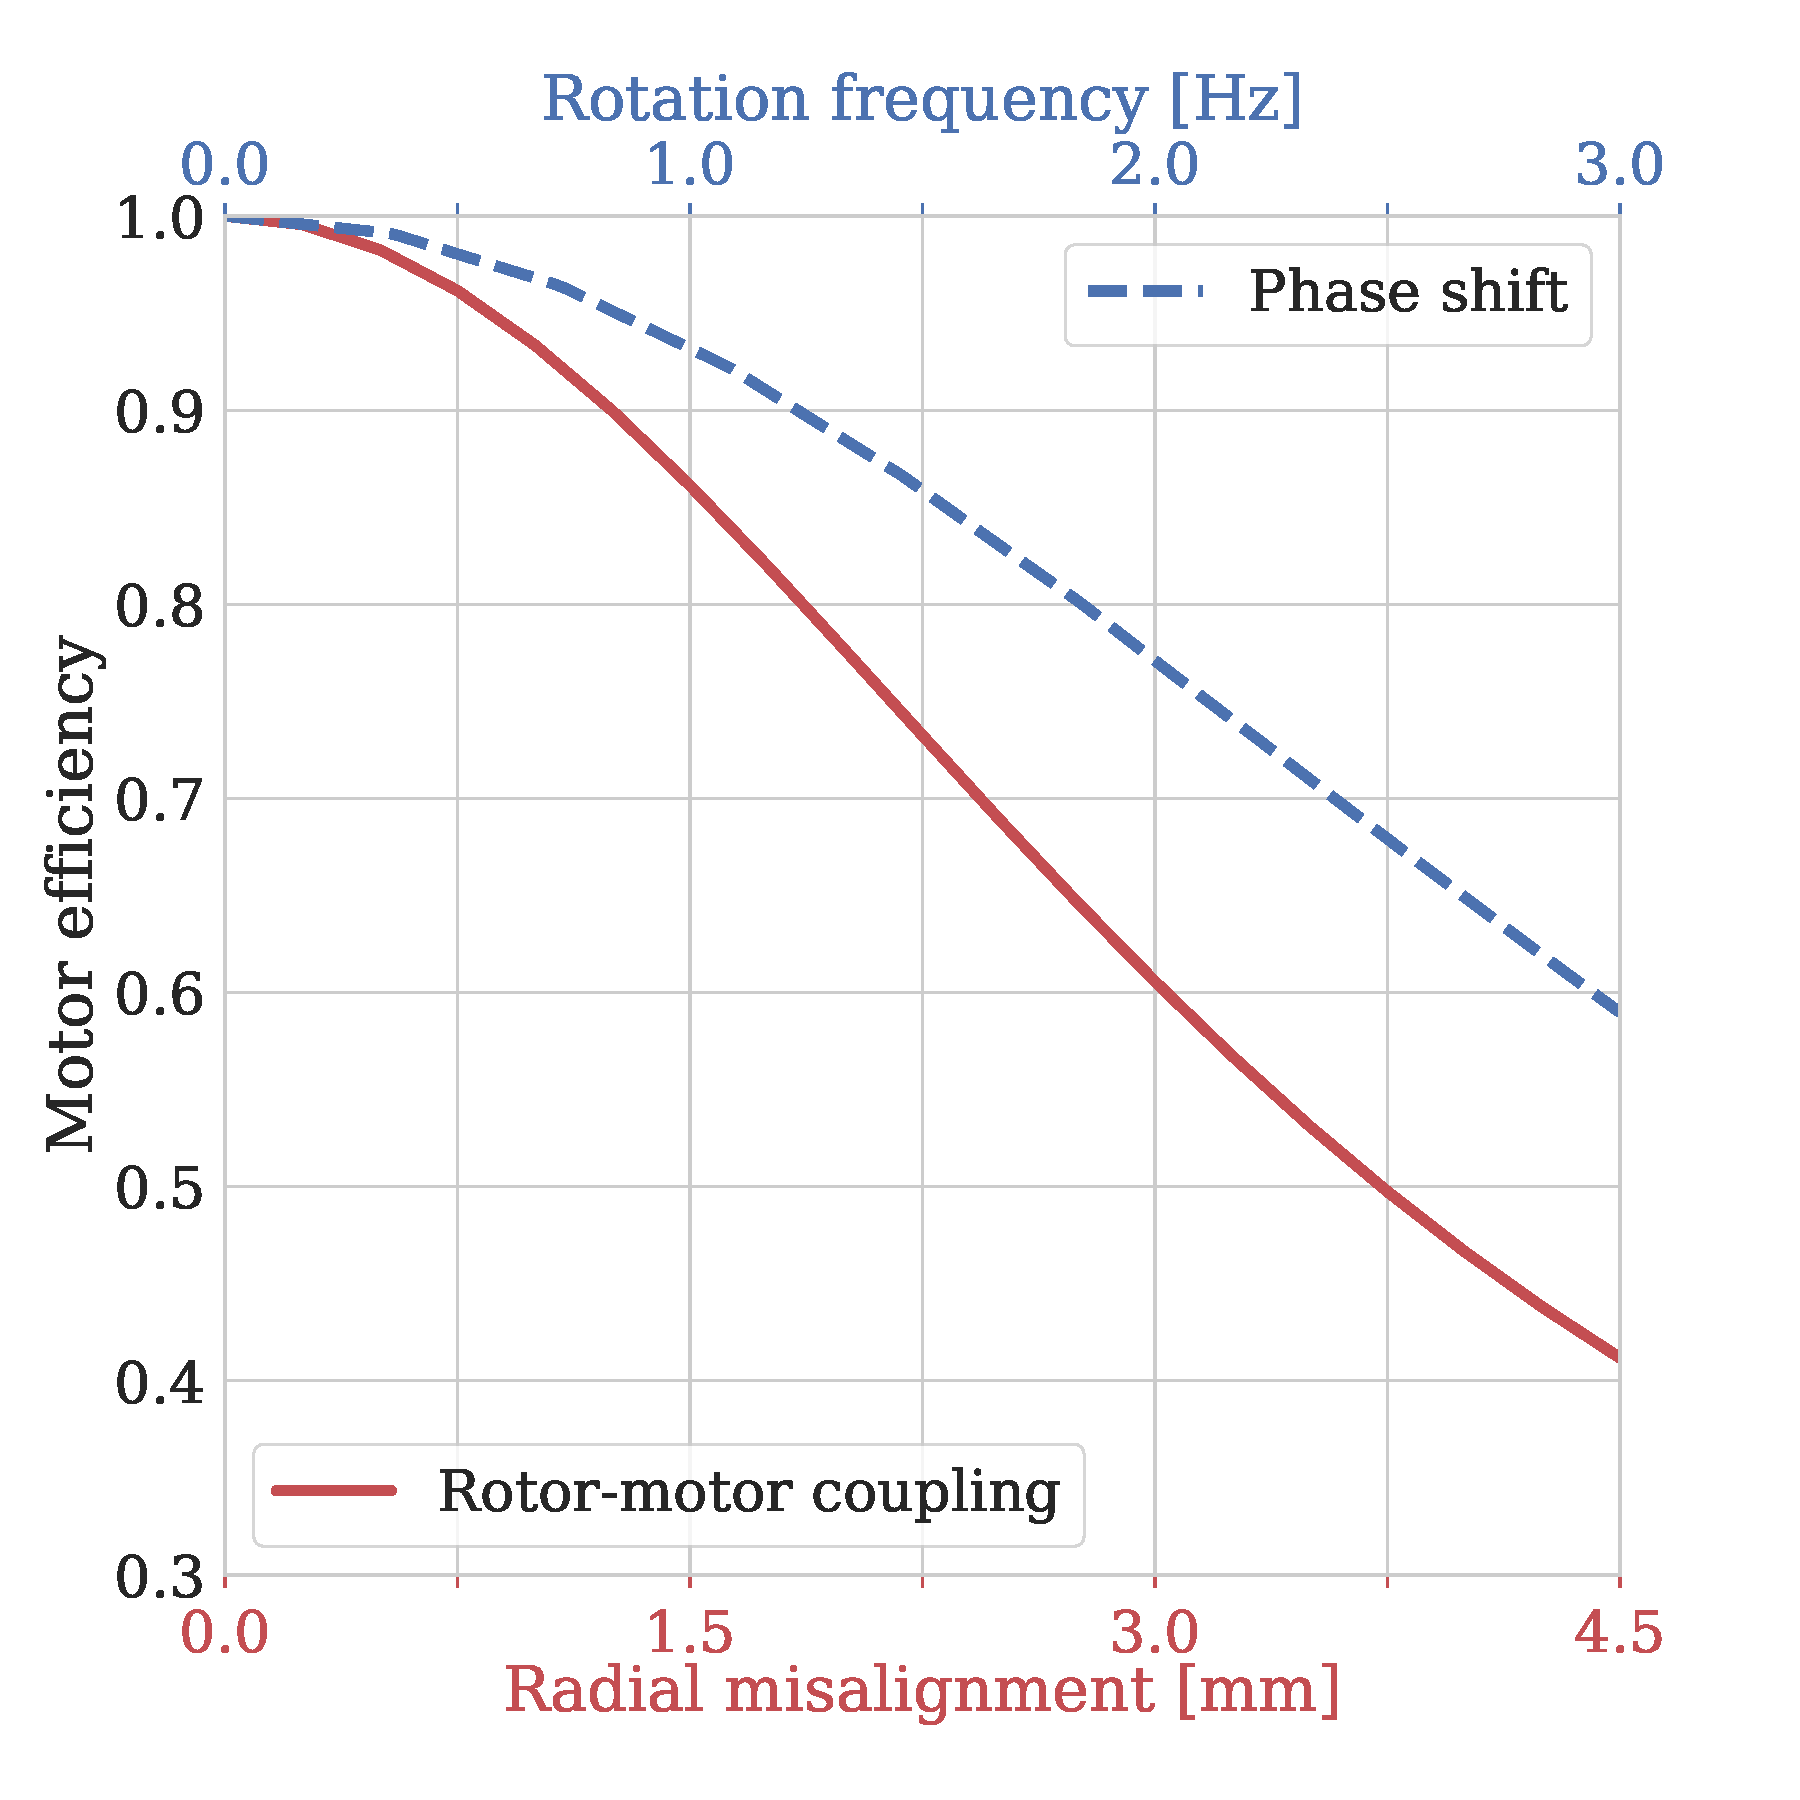
\includegraphics[width=0.5\linewidth, trim=0.5cm 1cm 2cm 1cm]{CHWPDesign/Figures/motorEff_vs_misalignment_HWPfreq.pdf}
    \caption{CHWP motor efficiency vs. the rotor's radial misalignment to the motor solenoids and the rotor's rotation frequency. The PB-2b rotor alignment tolerance is <~2~mm, limiting positional efficiency loss to <~20\%. At 2~Hz rotation, the phase-delay efficiency loss is $\approx$~20\%.}
    \label{fig:motor_eff}
\end{figure}

%%%%%%%%%%%%%%%%%%%%%%%%%%%%%%%%
%%%%%%%%%%%%%%%%%%%%%%%%%%%%%%%%
%%%%%%%%%%%%%%%%%%%%%%%%%%%%%%%%

\section{Angle encoder}
\label{sec:angle_encoder}

The rotor angle is measured by an incremental encoder that uses much of the same infrastructure as the motor encoder (see Section~\ref{sec:motor_design}). The angle encoder's signal schematic is shown as part of Figure~\ref{fig:motor_driver_schematic}, and its cryogenic components are shown in Figure~\ref{fig:motor_mech_assy}. On each encoder read head, two LED-PD pairs peer through $570 - 1 = 569$ slots on the slotted encoder plate with one missing slot to mark the rotor's absolute position. During 2~Hz continuous rotation, the PD photocurrents are chopped at 1.14~kHz, are digitized on the driver board, are opto-isolated to 3.3~V, and are processed by a microcontroller unit (MCU). The two angle encoder LED-PD pairs are offset by half a slot width, enabling quadrature readout to monitor rotation direction.

The MCU is a BeagleBone Black (BBB),\footnote{Beagle Board: https://beagleboard.org/black} which houses two programmable real-time units (PRUs) and an on-board CPU running Linux. The PRU is a lightweight, low-latency processing unit specifically designed to handle single-threaded inputs, making it ideal for angle encoding. One PRU polls the angle encoder signal and uses a 200~MHz clock\footnote{Specifically, both PRUs access the industrial Ethernet protocol (IEP) timer.} to timestamp each rising and falling edge. Simultaneously, a second PRU polls and decodes a GPS-synchronous inter-range instrumentation group B code (IRIG-B)\footnote{Spectrum Instruments TM-4: http://www.spectruminstruments.net/} PWM waveform using the same 200~MHz clock. The encoder and IRIG clock values are written to a shared memory buffer that is periodically emptied by the CPU, which in turn sends IPv4 data packets to an external computer. During post-processing, the rotor angle is reconstructed using the missing reference slot and is interpolated to IRIG time using the MCU clock values. This time-ordered CHWP angle data can then be used to demodulate the detectors, which are also synchronized to IRIG.

While the CHWP angle jitter requirement is $\ll$~$3$~$\mathrm{\mu rad / \sqrt{Hz}}$, the encoder only has a resolution of 5~mrad, necessitating precise interpolation between ticks on the slotted encoder plate. Such an encoding scheme is feasible because the CHWP rotation is very smooth and the encoder is high-signal-to-noise, enabling clean angle reconstruction (see Sections~\ref{sec:pb2a_chwp_evaluation_continuous_rotation} and~\ref{sec:pb2b_chwp_evaluation_encoder_jitter}).

%%%%%%%%%%%%%%%%%%%%%%%%%%%%%%%%
%%%%%%%%%%%%%%%%%%%%%%%%%%%%%%%%
%%%%%%%%%%%%%%%%%%%%%%%%%%%%%%%%

\section{Thermal design}
\label{sec:thermal_design}

The effectiveness of the CHWP system depends centrally on its thermal performance. As shown in Figure~\ref{fig:pb2b_chwp_in_ot_cad:b}, the CHWP is located on the 50~K stage, which is cooled by the first stage of the optics tube's PTR. The rotor is shielded from sky-side radiation by the vacuum window, RT-MLI, and IRF, and it floats between the IRF and the field lens. As discussed in Section~\ref{sec:chwp_design_requirements}, the primary objective of the CHWP thermal design is to minimally impact both the 4~K and 50~K stage temperatures with respect to those of the heritage PB-2b configuration.

\begin{figure}[!t]
    \centering
    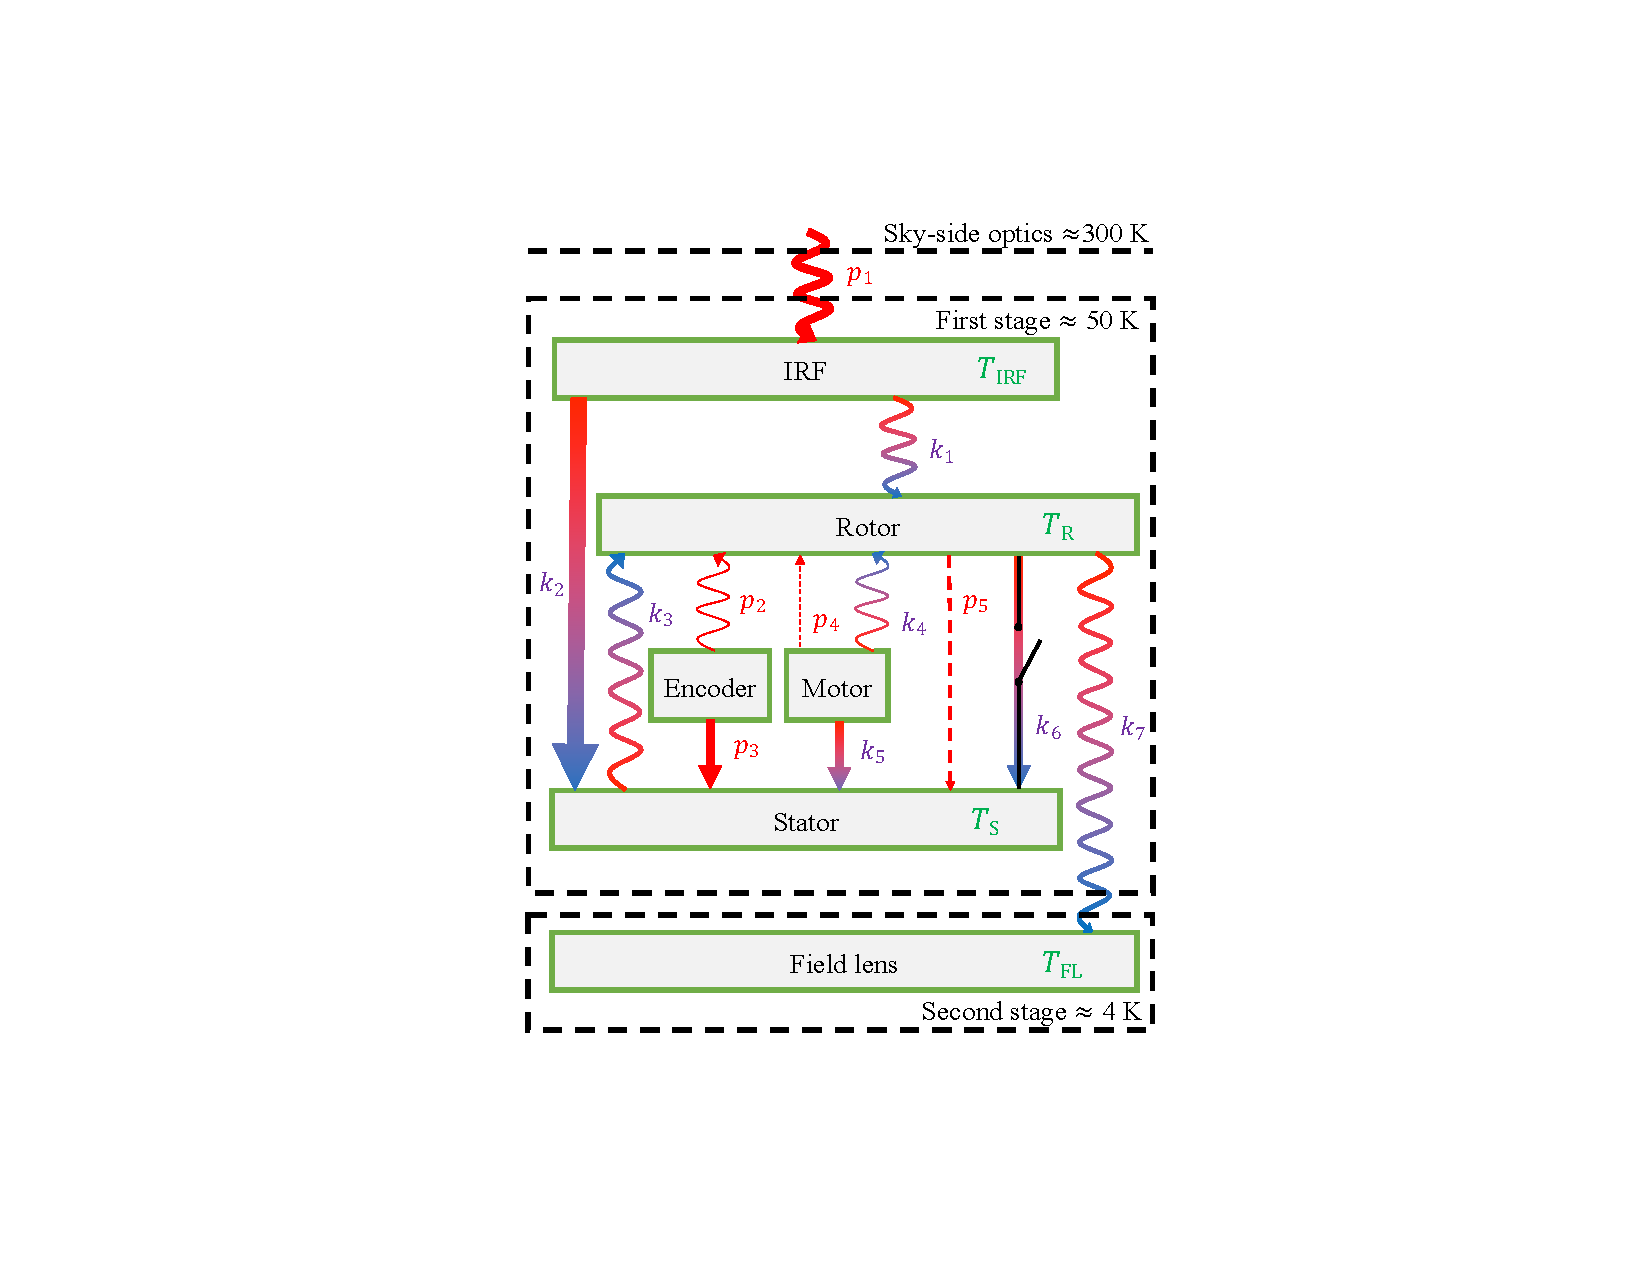
\includegraphics[width=0.7\linewidth, trim=8.5cm 4cm 8cm 3cm, clip]{CHWPDesign/Figures/thermal_diagram.pdf}
    \caption{The CHWP thermal circuit during nominal operation. The squiggly lines represent radiative loads, the straight lines conductive loads, and the dotted lines dissipative loads. Loads labeled by $p$ represent constant power, while loads labeled with $k$ represent power that depends on operating temperatures. Each conductivity has a red-to-blue color gradient from hot to cold. The switched conductivity $k_{6}$ represents the gripper connection, which is closed when the rotor is gripped and open when it is not. The lines' thicknesses show the relative magnitudes of the various contributions but are not to scale and are intended only as a visual guide. The IRF ($T_{\mathrm{IRF}}$), rotor ($T_{\mathrm{R}}$), stator ($T_{\mathrm{S}}$), and field lens ($T_{\mathrm{FL}}$) temperatures are the system's merit figures. The measured and calculated values for each symbol are given in Tab.~\ref{tab:thermal_values}.}
    \label{fig:thermal_diagram}
\end{figure}

\begin{table}
\caption{\label{tab:thermal_values} Parameter definitions and values for Fig.~\ref{fig:thermal_diagram}. The bold values are measured, while the non-bold values are estimates. The error bars represent some combination of uncertainties in the calculation or measurement as well as configurational variations.}
\centering
\begin{tabu}{| l | p{10cm} | r |}
    \hline
    Symbol & Description & Value \\
    \hline
    \hline
    $p_{1}$ & Radiative load from 300~K onto the IRF, including that of the sky, window, and RT-MLI & 17 $\pm$ 5 W \\
    \hline
    $p_{2}$ & Radiative load from the encoder LEDs onto the rotor & 10 $\pm$ 3 mW \\
    \hline
    $p_{3}$ & Power dissipated by the encoder LEDs onto the stator & 0.8 $\pm$ 0.2 W\\
    \hline
    $p_{4}$ & Eddy current and hysteresis dissipation onto the rotor due to the motor's oscillating magnetic field  & $<$~1 mW \\
    \hline
    $p_{5}$ & Rotor frictional dissipation during 2~Hz rotation & \textbf{80 $\pm$ 10 mW} \\
    \hline
    $k_{1}$ & Radiative coupling between the IRF and the rotor & 7 $\pm$ 2 mW/K \\
    \hline
    $k_{2}$ & Conductivity between the IRF and the stator & \textbf{2.5 $\pm$ 0.3 W/K} \\
    \hline
    $k_{3}$ & Radiative coupling between the stator and the rotor & 5 $\pm$ 2 mW/K \\
    \hline
    $k_{4}$ & Radiative coupling between the solenoid array and the rotor & $<$~1 mW/K \\
    \hline
    $k_{5}$ & Conductivity between the motor solenoids and the stator & \textbf{0.8 $\pm$ 0.1 W/K} \\
    \hline
    $k_{6}$ & Conductivity between the rotor and the stator via the gripper & \textbf{0.7 $\pm$  0.1 W/K} \\
    \hline
    $k_{7}$ & Radiative coupling between rotor and the field lens & 5 $\pm$ 1 mW/K \\
    \hline
\end{tabu}
\end{table}

When the rotor is stationary, loading on the 4~K stage is lower than in the heritage system. The IRF transmits non-negligibly $\lesssim$~2~THz \cite{inoue_cryogenic_2014}, and when present, the CHWP's sapphire stack absorbs $>$~90\% of this leaked sky-side power, keeping it from reaching the field lens. Additionally, because the rotor is floating, it acts as multi-layer insulation (MLI), reducing the 4~K load further. When the rotor is spinning, however, the solenoids, LEDs, and rotor generate heat, and if these loads warm the 50~K stage or rotor too much, 4~K improvements could be negated. Therefore, the CHWP design focuses on limiting 50~K dissipation and on keeping the rotor cool. 

We use an analytic simulation to predict rotor temperature and CHWP-induced power on the 50~K and 4~K stages during continuous operation in the field. Figure~\ref{fig:thermal_diagram} shows a schematic for the model, and Table~\ref{tab:thermal_values} shows the measured and calculated values for the schematic. The errors on the measured values contain both measurement and configurational uncertainties, while the errors on the calculated values are driven by uncertainties in the assumptions. We find that the most important contributions to the results shown in Figures~\ref{fig:rotor_temp} and~\ref{fig:hwp_stability} are the IRF temperature, 50~K stage temperature, and the IR emissivity of the IRF and CHWP sapphire stack.
 
The CHWP is an 11.4~mm thick stack of three sapphire windows. At 50 K, the sapphire stack has an emissivity of 0.95 at $\sim$~3~THz \cite{oxford_instruments_windows_nodate}, and therefore the CHWP rotor absorbs IR radiation efficiently despite its AR coating. The dominant sources of radiative transfer to and from the rotor are the IRF, stator, and field lens. The IRF is heat-strapped to its fixture using 24 1~mm thick, 50~mm wide, 20~mm long flexible ribbons of 99.9999\% pure aluminum, which have superior conductivity between 100$\sim$50 K \cite{Woodcraft2005}, are malleable enough to engage the alumina surface without thermal grease, and are flexible enough to absorb differential thermal contraction between the IRF and its aluminum fixture. The IRF fixture is machined from aluminum 1100 and is bolted to six 90~mm tall, titanium-helicoiled OFHC copper towers (see Figure~\ref{fig:chwp_tabletop}), which provide a thermal path to the stator baseplate. The measured conductivity between the IRF and the stator baseplate is $k_{2} = 2.5$~W/K. During laboratory testing with a thick window and no AR coatings (see Section~\ref{sec:pb2a_chwp_evaluation_thermal_impact}), we see an IRF temperature $\approx$~5~K warmer than the 50~K stage, suggesting a $\approx$~13~W sky-side load, which is slightly less than the model's expectation but within its $1 \sigma$ uncertainty.

The sky-side power leaked through the IRF depends on its AR coating. We assume in this paper that the IRF and CHWP sapphire stack are coated with an epoxy-based ARC \cite{rosen_epoxy-based_2013}, which has a non-negligible transmissivity $\lesssim$~2~THz \cite{halpern_far_1986}. Using the effective temperature of a six-layer RT-MLI stack \cite{choi_radio-transparent_2013} and the transmission spectra for Stycast-coated alumina \cite{inoue_cryogenic_2014}, we estimate that $\approx 60 \; \pm \; 10$~mW of sky-side power leaks through the IRF onto the rotor (or, in the heritage PB-2b configuration without the CHWP, onto the field lens).
 
The stator baseplate is made from aluminum 1100, houses the motor and encoder, and includes a 3~mm thick 50~K shield (see Figure~\ref{fig:gripper_assy}) that encloses the CHWP assembly. The inner wall of the 50~K shield is coated with carbon-loaded Stycast \cite{persky_review_1999} and is intended to absorb any 300~K photons that leak into the CHWP cavity through the gripper ports. The 50 K shield is attached to the stator baseplate by only sixteen bolts, and therefore its temperature is typically $\approx$~5~K higher than that of the baseplate. The radiative coupling between the stator and the rotor is similar to that between the IRF and the rotor.
 
The encoder consists of two read heads, each with a set of five LEDs shining through the slotted encoder plate onto five photodiodes. At 50~K, the LEDs are current biased with 30-50~mA at 1.8~V, and therefore the power dissipated by each read head is 300$\sim$500 mW. We attach each read head to the stator baseplate using four 6~mm diameter aluminum 6061 standoffs with polished ends and interfaced with thermal grease,\footnote{Apiezon N Grease: https://www.apiezon.com/} and the estimated read-head warm-up is $<$~1~K. The LEDs also shine onto the rotor's slotted encoder plate, whose slit patterns have 50\% duty cycles. The LED emits between 900 and 960 nm, and its beam has a peak intensity of 35 mW/sr at 50 mA bias with a full-width-half-max of $\pm \; 7^{\circ}$. In order to limit stray read-head emission, each LED is collimated by a 1~mm wide, 3~mm deep hole that truncates its beam at $\pm \; 10^{\circ}$. Upon integrating these LED beams over the collimation holes, the estimated loading on the rotor from both encoder read heads is $10 \; \pm \; 3$~mW.
 
During 2~Hz rotation, the motor solenoids carry an RMS current of $\approx$~20~mA, generating a peak-to-peak magnetic field of $\approx$~20~G. The field is generated by a 38$f_{\mathrm{HWP}}$, $V_{\mathrm{D}}\; \approx \; 12 \mathrm{V}$ square-wave (at $f_{\mathrm{HWP}} \approx 2$~Hz), which is low-pass filtered above $\approx$ 300~Hz. To keep the coils cool, we epoxy\footnote{Stycast 2850FT: https://www.henkel-adhesives.com/us/en/product/potting-compounds/loctite\_stycast\_2850ft.html} them to their cores, providing a $7 \; \pm \; 2$~mW/K conductive path to the stator. At 50~K, each coil's resistance is $\approx \; 3 \; \mathrm{\Omega}$, dissipating $\approx \; 1$~mW per coil during continuous rotation. This dissipation warms the coils $<$~1~K, and their radiative coupling to the rotor is $<$~1~mW/K. In order to minimize eddy current dissipation on the rotor due to the motor's oscillating magnetic field, the encoder plate is made of G10, limiting eddy losses on the rotor to the sprocket ring. Electromagnetic dissipation within low-carbon steel at $\sim$~10~G and $\sim$~100~Hz frequencies induces $<$~1~mW of heating on the rotor.

The field lens is $\approx$~50~mm thick and is therefore assumed to have an IR emissivity of 1 for all calculations. Its coupling to the rotor is determined purely by the CHWP aperture diameter and the field-lens view factor and is calculated to be $5 \; \pm \; 1$~mW/K.

Assuming the model presented in Figure~\ref{fig:thermal_diagram} and Table~\ref{tab:thermal_values},  Figure~\ref{fig:rotor_temp} shows the rotor temperature and the CHWP-induced load on the field lens as a function of excess power on the rotor, where ``excess'' is defined as that which is beyond the model's prediction. The expected rotor temperature is 52~to~54 K and the expected CHWP-induced field lens load is $-70$~to~$-10$~mW with respect to the heritage configuration. CHWP-induced power on the field lens is $<$~0~mW at 85\% confidence when the rotor is $<$~55~K, which motivates the rotor temperature requirement presented in Section~\ref{sec:thermal_requirements}. CHWP-induced power on the 50~K stage is $<$~1.3~W at 85\% confidence and is nearly independent of rotor temperature.

\begin{figure}[!t]
    \centering
    \subfloat[\label{fig:rotor_temp:a}]{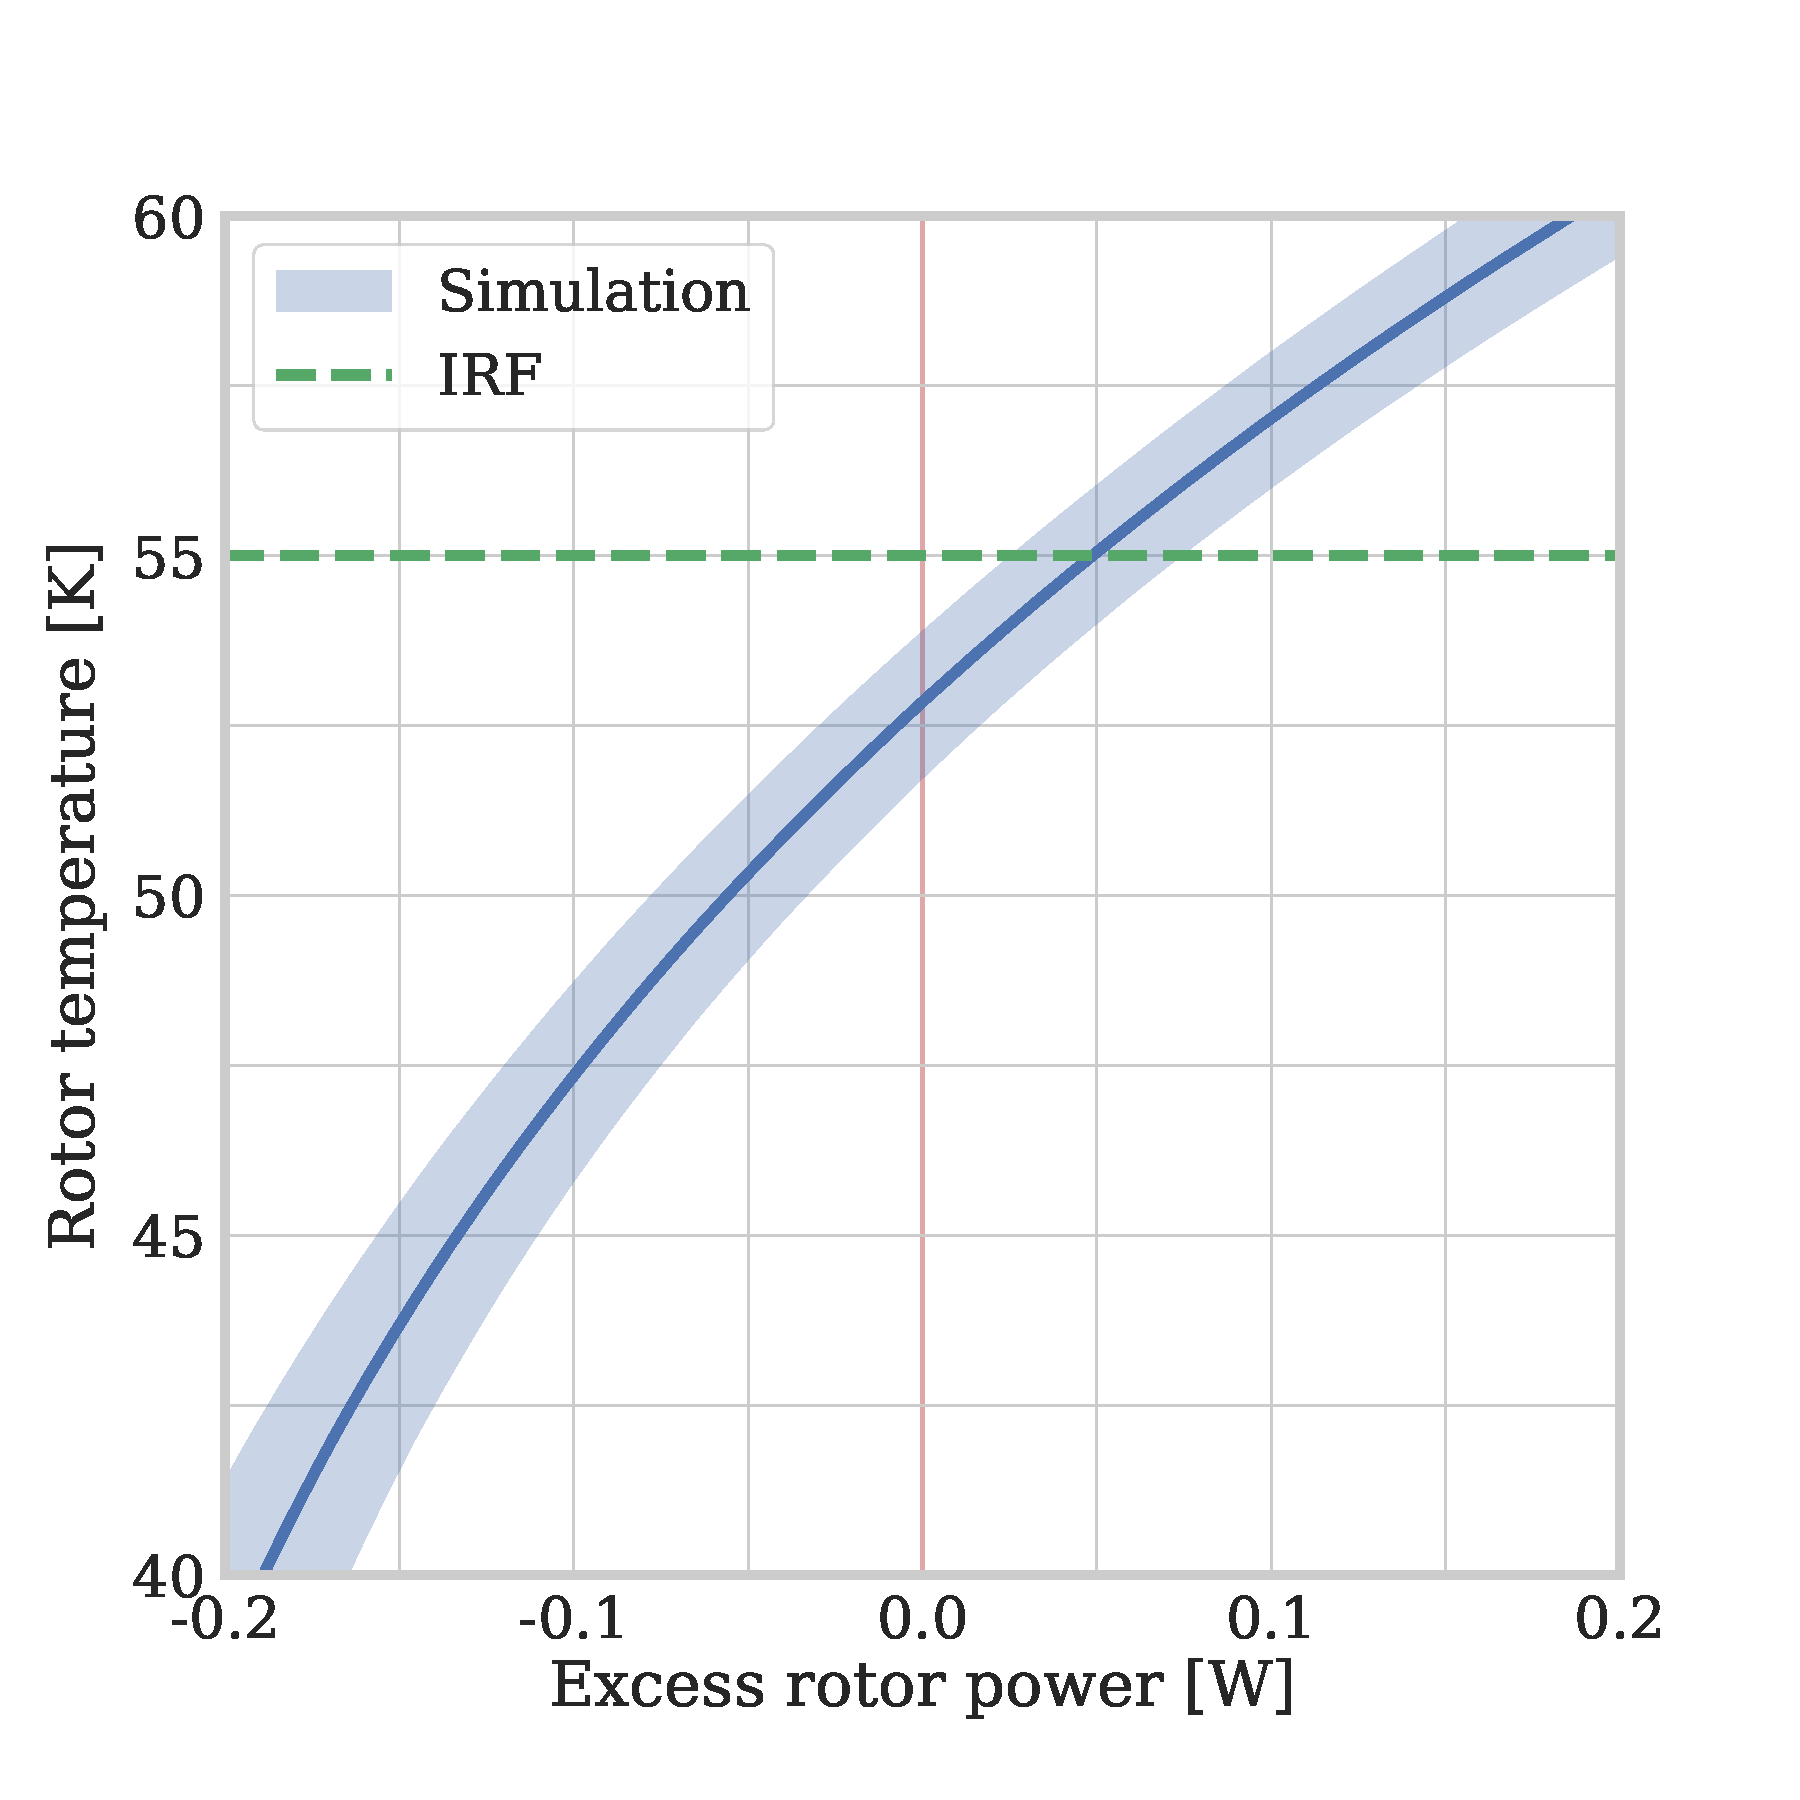
\includegraphics[width=0.5\linewidth, trim=0.5cm 0.5cm 1.3cm 2.5cm, clip]{CHWPDesign/Figures/rotorTemp_vs_rotorPower.pdf}}
    \subfloat[\label{fig:rotor_temp:b}]{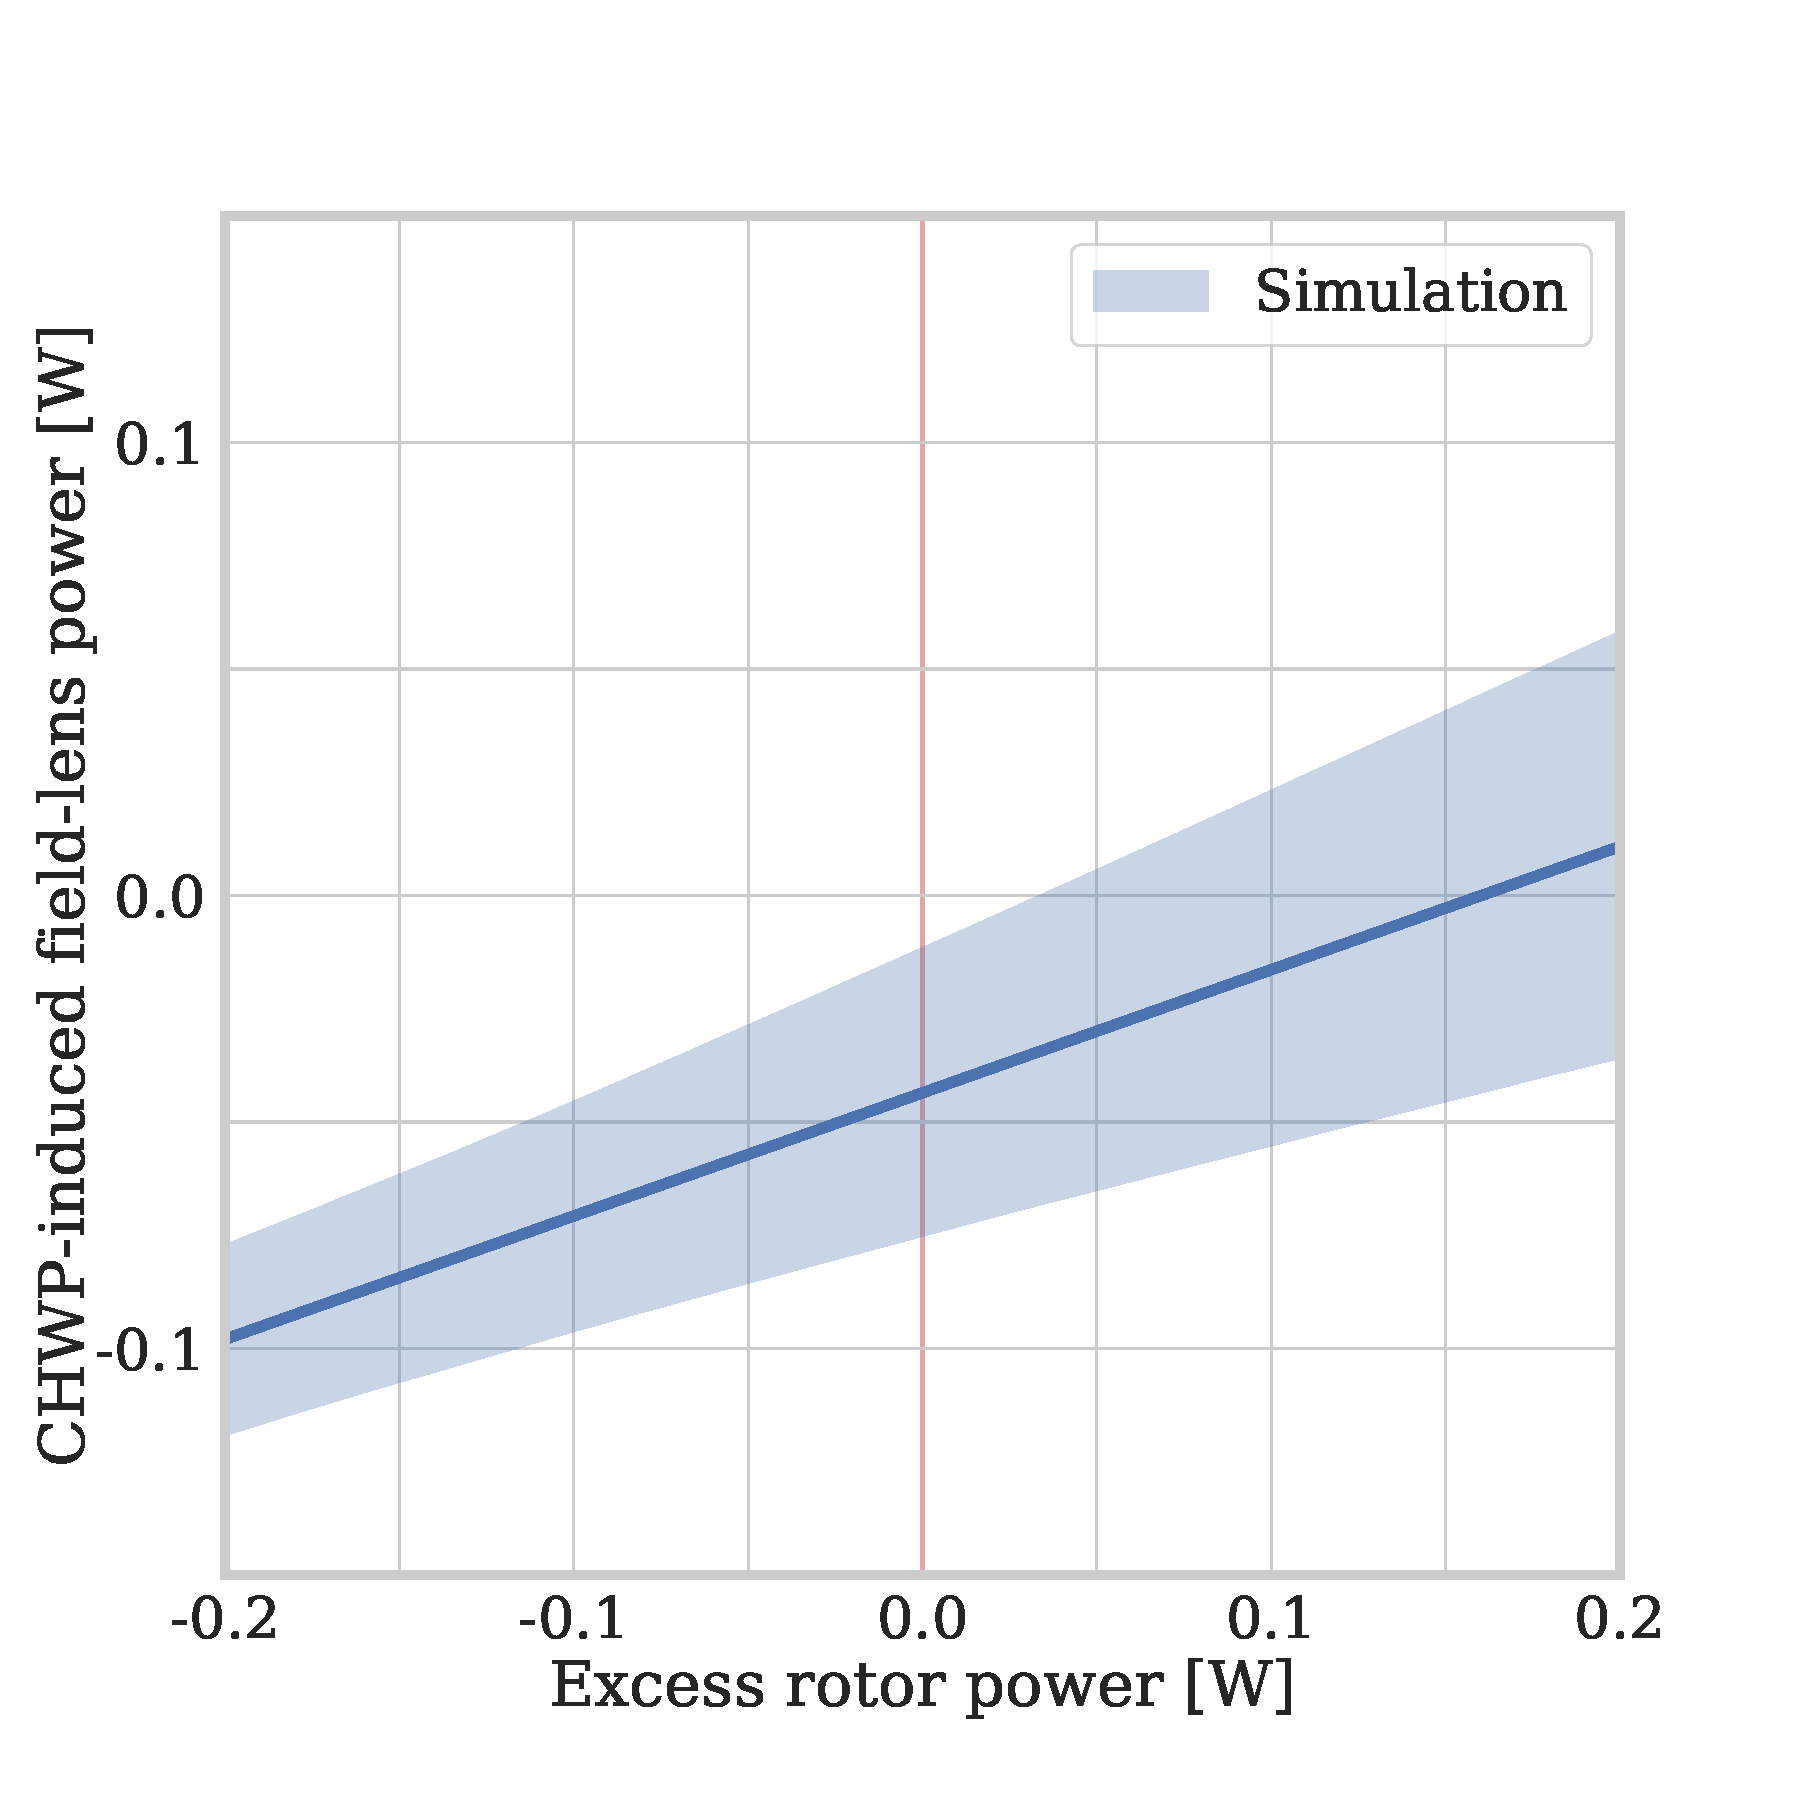
\includegraphics[width=0.5\linewidth, trim=-0.5cm 0.5cm 2.3cm 2.5cm, clip]{CHWPDesign/Figures/fieldLensPower_vs_rotorPower.pdf}}
    \caption{Rotor temperature (left panel) and CHWP-induced power on the field lens (right panel) as a function of excess, unmodeled power on the rotor. The solid blue line represents the median, while the shaded regions denote one-sigma uncertainties. Each plot's y-intercept gives the modeled expectation, and the IRF is assumed to be 55~K.}
    \label{fig:rotor_temp}
\end{figure}

%%%%%%%%%%%%%%%%%%%%%%%%%%%%%%%%
%%%%%%%%%%%%%%%%%%%%%%%%%%%%%%%%

\subsection{Rotor thermometry}
\label{sec:rotor_thermometry}

Two modes are used to monitor the rotor's temperature. First, when the rotor is gripped, four spring-loaded contacts on each gripper finger touch four flex-circuit traces on the rotor stage (see Section~\ref{sec:gripper_design}). These traces are soldered to a four-wire silicon diode thermometer, which is varnished to the sapphire stack's cradle. While only one contact current biases the diode, all three probe the diode's voltage; therefore this flex-circuit thermometry is also a touch-sensing system used to verify the fit between the gripper's copper wedges and the rotor stage's triangular groove.

Second, during continuous rotation, we use the ring magnet as a thermometer. Neodymium has a temperature-dependent magnetic field\footnote{Neodymium magnetization: \\ http://spontaneousmaterials.com/Papers/TN\_0302.pdf} that generates a $\sim$~1~G/K variation $\approx$~5~mm from the ring magnet's face \cite{Sakurai2018}. We varnish a 1~mm~thick cryogenic Hall sensor\footnote{Lakeshore HGCT-3020: https://shop.lakeshore.com/} to the surface of the YBCO and monitor long-time-scale changes in the ring magnet's average field. Limited by degeneracy with rotor position, the sensitivity of this scheme is a few K, and therefore, Hall-sensor monitoring is intended to flag thermal events rather than subtract rotor temperature drifts from detector data. If the need to re-calibrate the Hall-sensor output arises, the CHWP can be stopped and gripped to cross-check the diode thermometer via the touch probes.

%%%%%%%%%%%%%%%%%%%%%%%%%%%%%%%%
%%%%%%%%%%%%%%%%%%%%%%%%%%%%%%%%
%%%%%%%%%%%%%%%%%%%%%%%%%%%%%%%%

\section{Integration}
\label{sec:assembly_procedure}

The CHWP assembly is designed to be modular, allowing for seamless integration into a nearly-fully-assembled PB-2b receiver. As shown in Figure~\ref{fig:chwp_tabletop}, the CHWP assembles mostly on the benchtop, which facilitates a smooth integration into the receiver. To secure the rotor to the stator and keep the two concentric during installation, the rotor stage is bolted to three of the copper towers in Figure~\ref{fig:chwp_tabletop:b} using aluminum installation stanchions. Then, four handles are bolted to the top-most face of the rotor stage, which allows the assembly to be safely maneuvered. 

Figure~\ref{fig:pb2b_chwp_installation} shows the CHWP assembly being installed into the PB-2b optics tube, which is constructed from the ground towards the sky on a cart that can modulate the receiver's elevation. Straps are attached to the four handles, and a hoist lifts the CHWP above the receiver. Then, the CHWP is lowered and bolted onto the 50~K stage before the receiver is rotated to a horizontal position. At this point, the gripper subassemblies are installed, the retaining ring is added, and the IRF, RT-MLI, and vacuum window close the cryostat. 

The fact that the CHWP integrates into a nearly fully assembled receiver allowed the CHWP and receiver to be evaluated in parallel prior to full system validation. This implementation was inspired in part by the modularity of the PB-2a WHWP and is a major advantage of the CHWP design that accelerated the PB-2b commissioning process. The sapphire stack is also modular, enabling the AR coatings to be easily replaced in the field, if necessary.

\begin{figure}[!t]
    \centering
    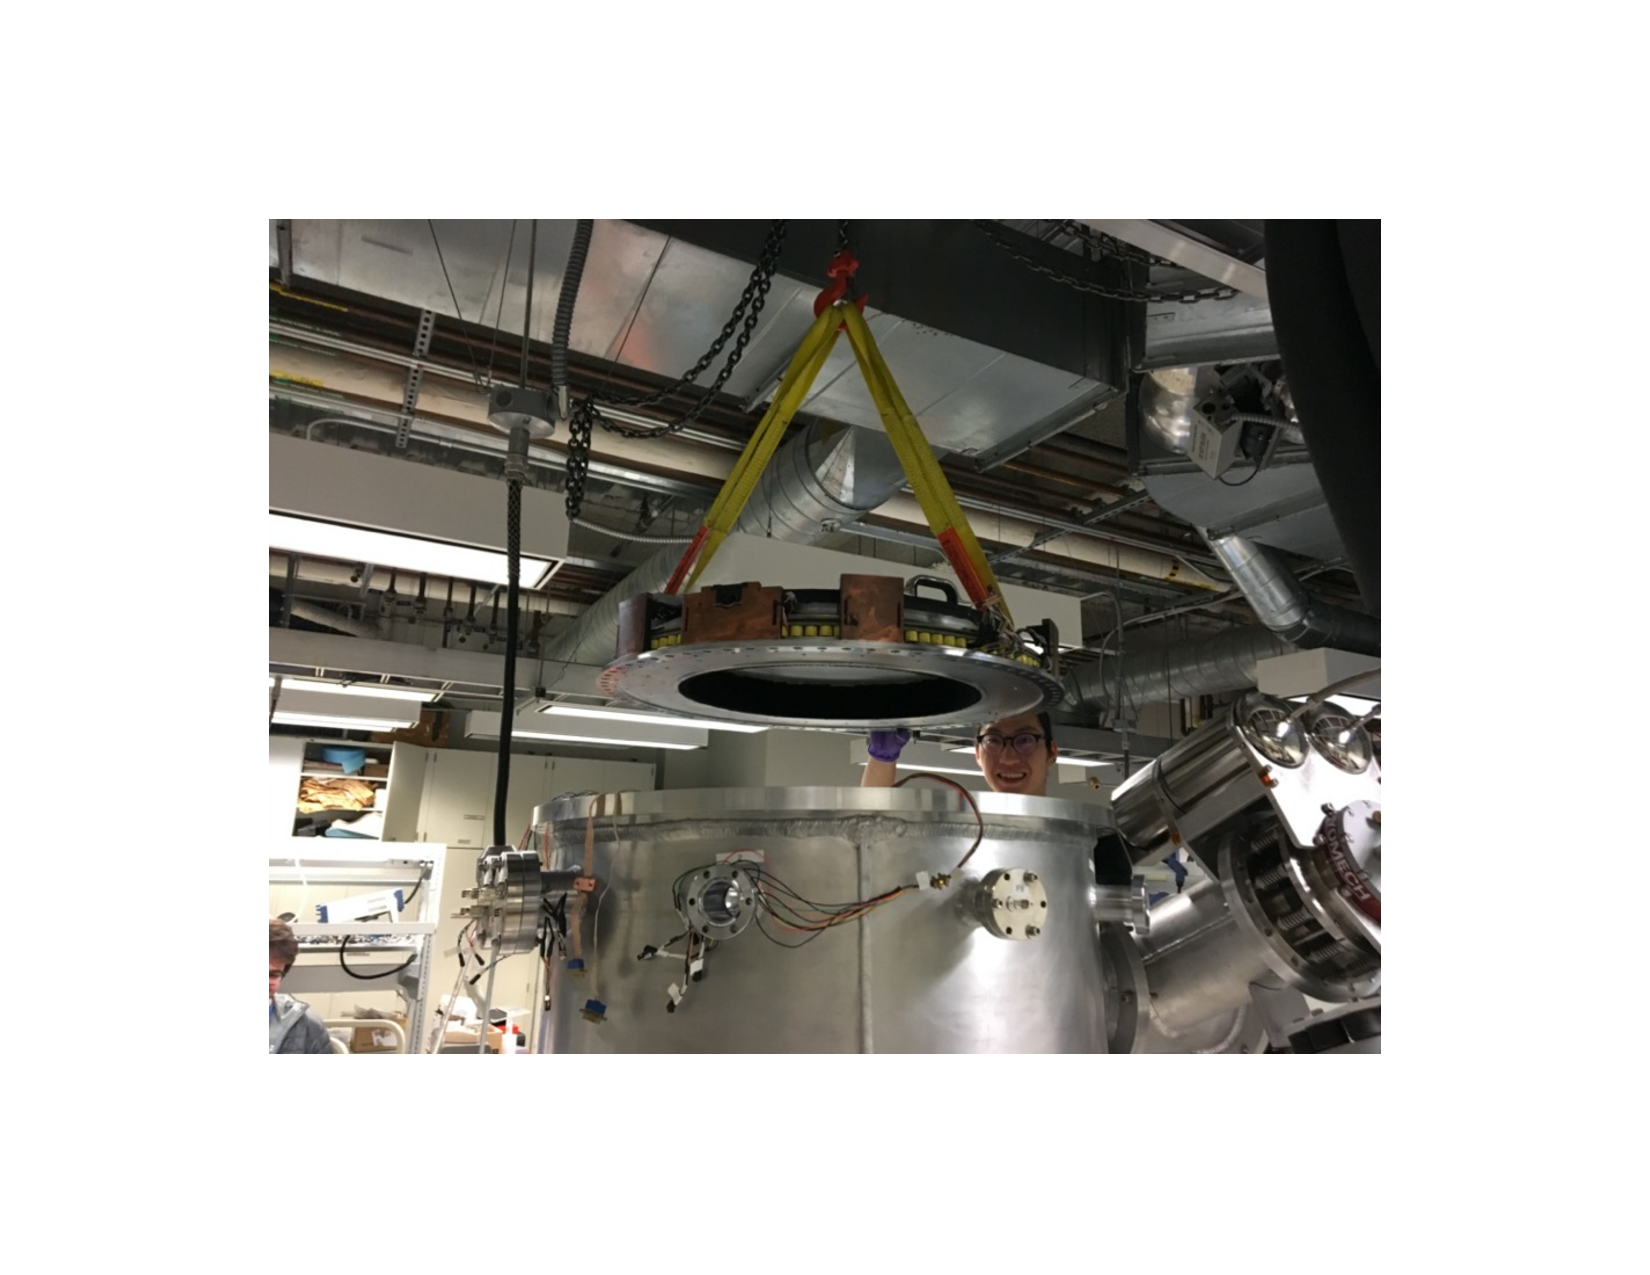
\includegraphics[width=0.7\linewidth, trim=4cm 4cm 4cm 4cm, clip]{CHWPDesign/Figures/pb2b_chwp_integration.pdf}
    \caption{The CHWP being installed into the PB-2b optics tube. The optics tube is constructed vertically on a cart, building from the focal plane towards the sky. The CHWP is one of the last elements to be installed and is hoisted using a series of handles that attach to the rotor stage. Once high enough, the CHWP is slowly lowered into the receiver and is bolted to the 50~K stage.}
    \label{fig:pb2b_chwp_installation}
\end{figure}